
% LaTeX file for a 1 page document
%\documentclass[12pt]{book}
\documentclass[12pt]{article}
\usepackage{graphicx,amsmath,hyperref,natbib}
\numberwithin{equation}{section}
\usepackage{enumitem}
\usepackage{url}
\usepackage[font=small,labelfont=bf]{caption}
\usepackage[]{sidecap}


% hyperref
\hypersetup{linktocpage}
\hypersetup{
    colorlinks,
    citecolor=blue,
    filecolor=blue,
    linkcolor=blue,
    urlcolor=blue
}

% journal defs
\def\araa{ARA\&A}             % Annual Review of Astron and Astrophys
\def\aap{A\&A}             % Annual Review of Astron and Astrophys
\def\apj{ApJ}

\def\exp{\mathrm{e}}
\def\dd{\mathrm{d}}
\def\Inu{\ensuremath{I_{\nu}}}
\def\jnu{\ensuremath{j_{\nu}}}
\def\Jnu{\ensuremath{J_{\nu}}}
\def\Bnu{\ensuremath{B_{\nu}}}
\def\Fnu{\ensuremath{F_{\nu}}}
\def\Snu{\ensuremath{S_{\nu}}}
\def\anu{\ensuremath{\alpha_{\nu}}}
\def\taunu{\ensuremath{\tau_{\nu}}}
\def\taumunu{\ensuremath{\tau_{\mu\nu}}}
\def\Fla{\ensuremath{F_{\lambda}}}

% magnitude stuff
\newcommand*{\logten}{\mathop{\log_{10}}}
\def\mA{\ensuremath{m_{\mathrm{A}}}}
\def\mB{\ensuremath{m_{\mathrm{B}}}}
\def\mC{\ensuremath{m_{\mathrm{C}}}}
\def\FA{\ensuremath{F_{\mathrm{A}}}}
\def\FB{\ensuremath{F_{\mathrm{B}}}}
\def\FV{\ensuremath{F^\mathrm{V}}}
\def\FC{\ensuremath{F^\mathrm{C}}}


\def\nelec{\ensuremath{n_\mathrm{e}}}
\def\Jbar{\ensuremath{\overline{J}_{\nu0}}}

% planck function
\def\Plancknu{\ensuremath{ \frac{2 h \nu^3}{c^2} \frac{1}{\exp^{h \nu / kT} -1}}}
\def\Planckla{\ensuremath{ \frac{2 h c^2}{\lambda^5} \frac{1}{\exp^{h c / \lambda kT} -1}}}

\def\Ila{\ensuremath{I_{\lambda}}}
\def\Bla{\ensuremath{B_{\lambda}}}

\def\Tb{\ensuremath{T_\mathrm{b}}}

\def\dO{\ensuremath{\dd \Omega}}
\def\ds{\ensuremath{\dd s}}
\def\dnu{\ensuremath{\dd \nu}}

% vector r and n
\def\vr{\ensuremath{\vec{r}}}
\def\vn{\ensuremath{\vec{n}}}
% unit n
\def\un{\ensuremath{\hat{n}}}
\def\uu{\ensuremath{\hat{u}}}
\def\uk{\ensuremath{\hat{k}}}
\def\ul{\ensuremath{\hat{l}}}

% Doppler width
\def\dnud{\ensuremath{\Delta \nu_\mathrm{D}}}
\def\dlad{\ensuremath{\Delta \lambda_\mathrm{D}}}

\newcommand{\be}{\begin{equation}}
\newcommand{\ee}{\end{equation}}
\newcommand{\bea}{\begin{eqnarray}}
\newcommand{\eea}{\end{eqnarray}}

%hydrogen particle density
\def\HII{H~II}

\def\nH{\ensuremath{n_\mathrm{H}}}
\def\nHI{\ensuremath{n_\mathrm{H \, I}}}
\def\nHII{\ensuremath{n_\mathrm{H\, II}}}

% electron mass
\def\me{\ensuremath{m_\mathrm{e}}}


% exercise macros
\newcommand{\rme}{{\rm e}}
\newcommand{\Fopp}{{F}_{\rm surf}}
\newcommand{\Fnuopp}{{F}_{\nu, {\rm surf}}}

\newcommand{\Rnu}{{\cal R}_\nu}
\newcommand{\Lnu}{L_\nu}
\newcommand\Izon{I^{\rm sun}}
\newcommand\Idet{I^{\rm det}}


\newcommand{\tnu}{\tau _\nu}
\newcommand{\anul}{\alpha _{\nu,l}}
\newcommand{\anuc}{\alpha _{\nu,c}}

\newcommand{\tot}{{\rm tot}}
\newcommand{\opp}{{\rm surf}}
\newcommand{\ff}{{\rm ff}}
\newcommand{\bb}{{\rm bb}}
\newcommand{\fb}{{\rm bf}}

\newcommand{\dt}{\dd t}
\newcommand\dOdet{\dO^{\rm det}}
\newcommand\dOzon{\dO^{\rm sun}}
\newcommand{\dOm}{\dd \Omega}
\newcommand{\dE}{\dd E}

\newcommand\qmax{{\theta_{\rm max}}}




% Commands

\newcommand{\figuur}[1]{\vspace{5 cm} \begin{center} Figuur #1 %
 \end{center} \vspace{2 ex}}

\newcommand{\opgave}[1]{\medbreak\item{\em #1}\par\nobreak\noindent\let\next}

\newcommand{\contvragen}{\setcounter{vraag}{\value{lastvraag}}}
\newcommand{\contsubvragen}{\setcounter{subvraag}{\value{lastsubvraag}}}

% Environments

\newcounter{vraag}	\newcounter{lastvraag}
\newenvironment{opgaven}%
    {\begin{list}{\arabic{vraag}.}{\usecounter{vraag}%
        \listparindent=\parindent \parsep=\parskip}}%
    {\setcounter{lastvraag}{\value{vraag}} \end{list}}

\newcounter{subvraag}	\newcounter{lastsubvraag}
\newenvironment{subvragen}%
    {\begin{list}{\alph{subvraag})}{\usecounter{subvraag}%
        \setlength{\rightmargin}{\leftmargin}}}%
    {\setcounter{lastsubvraag}{\value{subvraag}} \end{list}}

\newenvironment{dm}{\begin{displaymath}}{\end{displaymath}}



%%%%%%%%%%%%%%%%%%%%%%%%%%%%%%%%%%%%%%%%%%%%%%%%%%%%%%
\title{Astrophysical Spectra\\
         AS7006  - Spring 2017}
\author{Jorrit Leenaarts\\ jorrit.leenaarts@astro.su.se}
\date{}

%%%%%%%%%%%%%%%%%%%%%%%%%%%%%%%%%%%%%%%%%%%%%%%%%%%%%%
\begin{document}

\maketitle
\clearpage
\tableofcontents
\newpage

%%%%%%%%%%%%%%%%%%%%%%%%%%%%%%%%%%%%%%%%%%%%%%%%%%%%%%
\section*{Preface}
%%%%%%%%%%%%%%%%%%%%%%%%%%%%%%%%%%%%%%%%%%%%%%%%%%%%%%

These are the lecture notes for the course AS7006 - Astrophysical Spectra as given at the Department of Astronomy of Stockholm University. They are very much a work in progress and draw from many different sources. I want to give explicit credit to the most important ones here:
\begin{itemize}
\item Handwritten lecture notes by Alexis Brandecker
\item The lecture notes ``Radiative transfer in stellar atmospheres'' by Robert J. Rutten
\item The lecture notes ``The generation and transport of radiation'' by Robert J. Rutten
\item The book ``Radiative processes in astrophysics'' by George B. Rybicki and Alan P. Lightman.
\item The book ``Astrophysics of Gaseous Nebula and Active Galactic Nuclei'' by Donald E. Osterbrock
\end{itemize}
As these notes are a work in progress they will be continually updated during the course. Please send me an email if you find (or suspect) any errors.
\\
\\
Jorrit Leenaarts

\addcontentsline{toc}{section}{Preface}

%%%%%%%%%%%%%%%%%%%%%%%%%%%%%%%%%%%%%%%%%%%%%%%%%%%%%%
\newpage
\section{Introduction}
%%%%%%%%%%%%%%%%%%%%%%%%%%%%%%%%%%%%%%%%%%%%%%%%%%%%%%

Electromagnetic radiation (from now on just {\it radiation} or {\it photons})  has been and will remain the primary medium from which we obtain information from astrophysical objects. Cosmic rays -- which consist of protons, nuclei of heavier elements and electrons -- and  neutrinos are highly interesting other sources of information. They are however emitted by a much more restricted range of sources. Thus they cannot provide as wide a view of the Universe as radiation.

Photons do not decay, so they can carry information over literally cosmic distances as long as they are not absorbed by intervening matter. We can measure the direction, energy distribution as a function of wavelength (the {\it spectrum}) and direction of oscillation (the polarization state) of radiation and the time variation of these quantities, which all can be used to infer properties of astrophysical objects. 

Radiation is important for another reason: it influences the physical structure of many objects. It is for example an energy transport mechanism in stars, stellar winds can be driven by radiation pressure, starlight can heat the interstellar medium around them, and radiation was the primary contributor to the cosmic energy density during the radiation-dominated era in the early Universe.

Knowledge of the formation and transport of electromagnetic radiation is thus essential for an astrophysicist. In these notes we will have a closer look at a macroscopic description of radiation and its interaction with matter, with the main quantity being called {\it intensity}. We will also look at the detailed processes on the scale of atoms and molecules that can absorb and emit photons. We will then develop equations that couple the macroscopic description of radiation to the microscopic processes, so that we can describe the expected radiation given the properties of the emitting material, and conversely, given observed radiation, infer properties of the source.

%%%%%%%%%%%%%%%%%%%%%%%%%%%%%%%%%%%%%%%%%%%%%%%%%%%%%%
\newpage
\section{Solid angle}
%%%%%%%%%%%%%%%%%%%%%%%%%%%%%%%%%%%%%%%%%%%%%%%%%%%%%%

%%%%%%%%%%%%%%%%%%%%%%%%%%%%%%%%%%%%%%%%%%%%%%%%%%%%%%
\begin{figure*}
  \centering
  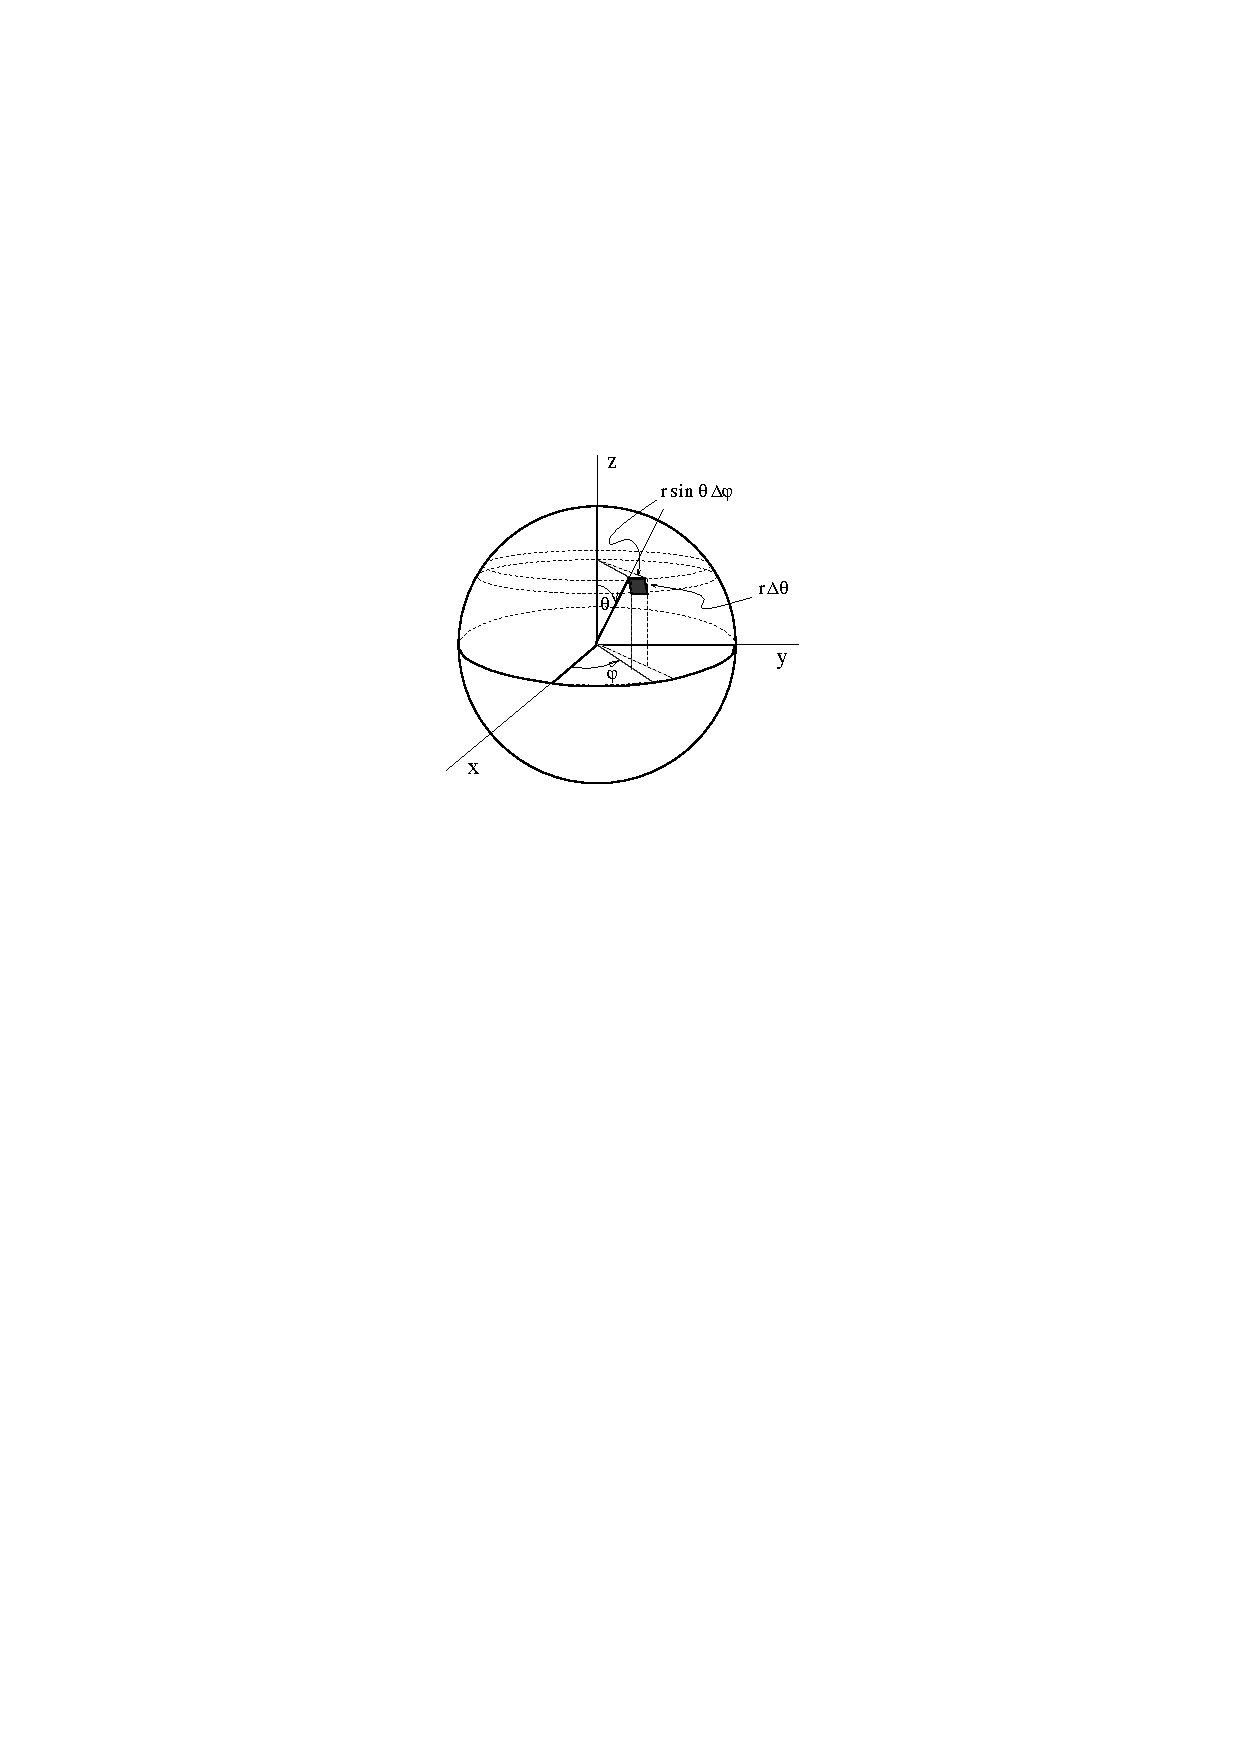
\includegraphics[width=8cm]{figs/fig_solid_angle}
  \caption{Solid angle in spherical coordinates. The area of the sphere with radius $r$ limited by $(\theta,\theta +\Delta\theta)$ and $(\phi,\phi +\Delta\phi)$ is $r^2 \sin{\theta} \, \Delta\theta \, \Delta\phi$ so that $\Delta \Omega = \sin{\theta}\, \Delta\theta \, \Delta\phi$. Adapted from \citet{2003rtsa.book.....R}.
  \label{fig:solid_angle}}
\end{figure*}
%%%%%%%%%%%%%%%%%%%%%%%%%%%%%%%%%%%%%%%%%%%%%%%%%%%%%%

In order to properly describe radiation, we need to introduce the concept of solid angle. This is best done in analogy with the concept of angle. The angular size of an object in a 2D plane is seen from the origin is the length of the projection of the object on the unit circle. This is of course how the radian is defined, and thus the maximum angular size of an object is:
\begin{equation}
\int_0^{2\pi} \dd \phi = 2\pi.
\end{equation}
Similarly we can define the solid angle as the surface area of the projection of an object on the unit sphere centred on the origin. So, an object that completely encloses the origin has a solid angle of
\be
\Omega = \int_0^{2\pi} \int_0^\pi \sin \theta \, \dd \theta\, \dd \phi = 4 \pi.
\ee
An infinitesimal solid angle $\dd \Omega$ can be interpreted as an infinitesimal surface on the unit sphere. In spherical coordinates:
\be
\dd \Omega = \sin \theta \,  \dd \theta \,  \dd \phi
\ee
We will use solid angle in the definition of intensity.

%%%%%%%%%%%%%%%%%%%%%%%%%%%%%%%%%%%%%%%%%%%%%%%%%%%%%%
\clearpage
\section{Radiation, intensity and flux}
%%%%%%%%%%%%%%%%%%%%%%%%%%%%%%%%%%%%%%%%%%%%%%%%%%%%%%

\subsection{Basic properties of radiation}

Radiation can be described as waves with different frequencies or as a stream of photons with different energies. In the wave description the frequency $\nu$, wavelength $\lambda$ and the speed of light in vacuum $c$ are related as
\be
\nu = \frac{c}{\lambda}.
\ee
The energy of a photon associated with a frequency $\nu$ is given by
\be
E = h \nu = \frac{hc}{\lambda},
\ee
where $h$ is Planck's constant. One can express photon energy or wave frequency with a formal temperature as well:
\be
T=\frac{E}{k} = \frac{h \nu}{k} = \frac{h c}{\lambda k},
\ee
where $k$ is Boltzmann's constant. 

In astronomy wavelengths are often expressed in units of \AA ngstr\"om (with symbol \AA), which is $10^{-10}$~m~$= 0.1$~nm.


\subsection{Definition of intensity}

%%%%%%%%%%%%%%%%%%%%%%%%%%%%%%%%%%%%%%%%%%%%%%%%%%%%%%
\begin{figure*}
  \centering
  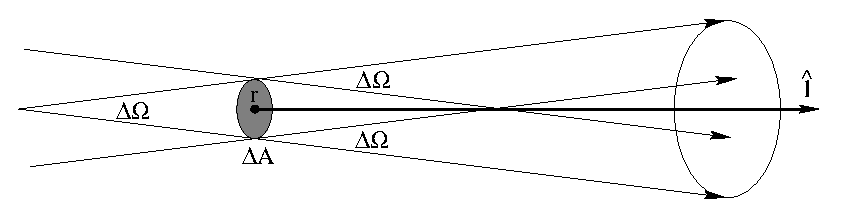
\includegraphics[width=12cm]{figs/intensity_def}
  \caption{Definition of intensity. Photons fly through the surface with area $\Delta A$ located at $\vec{r}$, in  a solid angle $\Delta \Omega$ around the direction $\hat{l}$. For simplicity the normal $\hat{n}$ of $\Delta A$ is taken parallel to $\hat{l}$ in this figure. The energy carried by these photons is proportional to $\Delta A$ and $\Delta \Omega$ if they are chosen so small that the radiation field is constant across these intervals.
  \label{fig:intensity_def}}
\end{figure*}
%%%%%%%%%%%%%%%%%%%%%%%%%%%%%%%%%%%%%%%%%%%%%%%%%%%%%%

The fundamental quantity with which we shall describe radiation is the intensity \Inu. It is defined so that for an area $\dd A$ with normal $\un$ and located at $\vec{r}$, the amount of energy transported through this surface between times $t$ and $t+\dd t$ in the frequency band $(\nu,\nu+\dd \nu)$ in a cone with solid angle $\dd \Omega$ around direction \ul\ is
\be
\dd E = \Inu(\vr, \ul ,t) \, (\hat{n} \cdot \hat{l}) \, \dd A \, \dd t \,  \dd \nu \,  \dd \Omega.
\ee 

The intensity can be expressed in various units, commonly used units are:
\bea 
\left[  \Inu  \right] & = &  \mathrm{W\ m}^{-2} \ \mathrm{Hz}^{-1} \ \mathrm{ster}^{-1} \\
\left[  \Inu \right]  & = &   \mathrm{erg}\ \mathrm{s}^{-1} \  \mathrm{cm}^{-2} \ \mathrm{Hz}^{-1} \ \mathrm{ster}^{-1} \\
 \left[    \Ila  \right]  &=&  \mathrm{W\ m}^{-2} \ \mathrm{m}^{-1} \ \mathrm{ster}^{-1} \label{eq:Ila_units}
\eea
In Eq.~\ref{eq:Ila_units} the intensity is defined for a wavelength band instead of a frequency band. The conversion from intensity per frequency unit to intensity per wavelength unit can be computed using the fact that the integration of intensity over a part of the spectrum must give the same answer, irrespective of whether we express it in frequency or wavelength units. Therefore
\bea
\int_{\nu1}^{\nu2} \Inu \, \dnu &=& \int_{\lambda(\nu1)}^{\lambda(\nu2)} \Inu \, \frac{\dnu}{\dd \lambda} \, \dd \lambda \nonumber \\
 & = & \int_{\lambda(\nu2)}^{\lambda(\nu1)} \Inu \, \frac{\nu^2}{c} \, \dd \lambda \nonumber \\
  & = &  \int_{\lambda(\nu2)}^{\lambda(\nu1)} \Ila \, \dd \lambda
\eea
Note that in the second equation the integration direction is reversed and so compensates for the minus sign in the derivative $\dnu / \dd \lambda$. The conversion of intensity from frequency to wavelength is thus given by:
\be
\Ila = \frac{\nu^2}{c} \Inu.
\ee

%%%%%%%%%%%%%%%%%%%%%%%%%%%%%%%%%%%%%%%%%%%%%%%%%%%%%%
\begin{figure*}
  \centering
  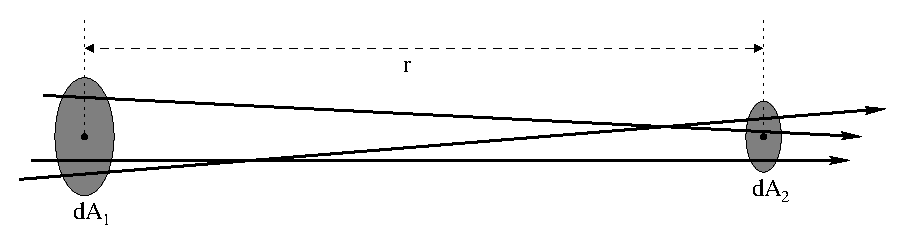
\includegraphics[width=12cm]{figs/intensity_conserved}
  \caption{Intensity is conserved along a ray.
  \label{fig:intensity_conserved}}
\end{figure*}
%%%%%%%%%%%%%%%%%%%%%%%%%%%%%%%%%%%%%%%%%%%%%%%%%%%%%%

The advantage of the intensity is that it is constant along a ray, and thus naturally accounts for the fact that photons to not decay. To see this we can  look at the energy carried by rays during a time interval $\dd t$ and a frequency band $\dd \nu$ passing through two surfaces $\dd A_1$ and $\dd A_2$ located a distance $r$ apart. Because photons do not decay, we know that the energies must be equal:
\be
\label{eq:Iconst}
\dd E_1 = {\Inu}_{,1} \, \dd A_1 \, \dd \Omega_1 \, \dd t  \, \dd \nu = \dd E_2 = {\Inu}_{,2} \, \dd A_2 \, \dd \Omega_2 \, \dd t \,  \, \dd \nu.
\ee
The solid angle that $\dd A_2$ subtends as seen from $\dd A_1$ is just
\be
\dd \Omega_1 = \frac{\dd A_2}{r^2},
\ee
and likewise
\be
\dd \Omega_2 = \frac{\dd A_1}{r^2}.
\ee
Substitution into Eq.~\ref{eq:Iconst} shows that
\be
{\Inu}_{,1} = {\Inu}_{,2}.
\ee
This means that intensity is conserved along a ray as long as no processes act to add or remove photons from a beam. An alternative expression of the same result is
\be
\frac{\dd \Inu}{\dd s} = 0,
\ee
where $s$ measures the length along the ray.

%%%%%%%%%%%%%%%%%%%%%%%%%%%%%%%%%%%%%%%%%%%%%%%%%%%%%%
\subsection{Additional radiation quantities}
%%%%%%%%%%%%%%%%%%%%%%%%%%%%%%%%%%%%%%%%%%%%%%%%%%%%%%

%%%%%%%%%%%%%%%%%%%%%%%%%%%%%%%%%%%%%%%%%%%%%%%%%%%%%%
\paragraph{Total intensity} 
If one integrates the intensity over frequency or wavelength one obtains the the total intensity:
\be
I(\vr,\ul,t) = \int_0^\infty \Inu \, \dd \nu = \int_0^\infty \Ila \, \dd \lambda
\ee
This is the total energy passing through a unit area per unit time per unit solid angle in the direction $\ul$. It has the following units:
\be 
\left[  I  \right] =  \mathrm{W\ m}^{-2} \ \mathrm{ster}^{-1}.
\ee

%%%%%%%%%%%%%%%%%%%%%%%%%%%%%%%%%%%%%%%%%%%%%%%%%%%%%%
\paragraph{Mean intensity} 
Integrating the intensity over all directions (all solid angles), and dividing by the maximum solid angle $4\pi$ yields the mean intensity
\be
\Jnu(\vr,t) =  \frac{1}{4 \pi}  \oint_\Omega \Inu \, \dO =  \frac{1}{4 \pi} \int_0^{2\pi} \int_0^\pi \Inu \, \sin{\theta} \, \dd \theta\, \dd \phi.
\ee
Mean intensity is a somewhat confusing name, as it is not obvious over which dependency the mean is computed: direction, frequency, time or location. A better name is angle-averaged intensity. The mean intensity has the same units as intensity:
\be
\left[  \Jnu  \right] =  \mathrm{W\ m}^{-2} \ \mathrm{Hz}^{-1} \ \mathrm{ster}^{-1}.
\ee

%%%%%%%%%%%%%%%%%%%%%%%%%%%%%%%%%%%%%%%%%%%%%%%%%%%%%%


%%%%%%%%%%%%%%%%%%%%%%%%%%%%%%%%%%%%%%%%%%%%%%%%%%%%%%
\begin{SCfigure*}
  \centering
  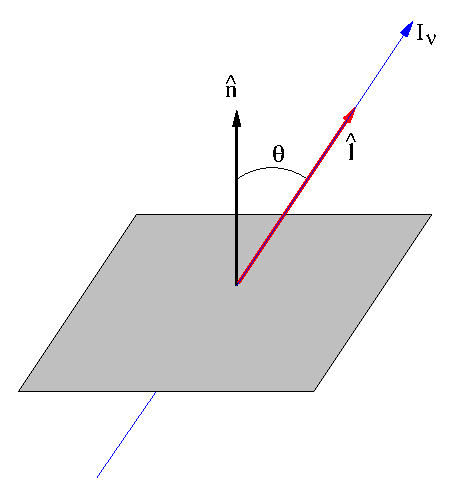
\includegraphics[width=6cm]{figs/flux_def}
  \caption{Definition of flux.
  \label{fig:flux_def}}
\end{SCfigure*}
%%%%%%%%%%%%%%%%%%%%%%%%%%%%%%%%%%%%%%%%%%%%%%%%%%%%%%


\paragraph{Flux} 
The monochromatic flux $\vec{F}_\nu$\ at a location \vr\ is defined as the net radiative energy flow at that location. It is a vector, it has a magnitude and a direction of the flow. Formally, it is defined as
\be
\vec{F}_\nu (\vr,t) = \oint \Inu(\vr,\ul,t) \, \ul \, \dO.
\ee

The flux in a specific direction \un\ is defined as the net flow of energy through a unit area placed perpendicular to \un\  per unit time (see Fig.~\ref{fig:flux_def}). It can be computed from the intensity as
\be \label{eq:flux_comp_def}
F_\nu (\vr, \un, t) = \oint \Inu (\vr,\ul,t) \, (\un \cdot \ul) \, \dO = \int_0^{2\pi} \int_0^\pi \Inu \cos \theta \sin \theta \, \dd \theta\, \dd \phi.
\ee 
The last equality is valid  using spherical coordinates with the $z$-axis aligned with \un. The units are:
\be
\left[ F_\nu  \right] = \mathrm{W\ m}^{-2} \ \mathrm{Hz}^{-1}.
\ee
Note the difference between intensity and flux. An isotropic radiation field (which means that $\Inu$ does not depend on the direction $\ul$) has no net energy flux, but a non-zero intensity. This can be seen by simply performing the integral in Eq.~\ref{eq:flux_comp_def} with constant $\Inu$:
\bea
F_\nu (\vr, \un, t) &=& \int_0^{2\pi} \int_0^\pi \Inu \cos \theta \sin \theta \, \dd \theta\, \dd \phi \nonumber \\ 
& = & 2\pi \Inu \int_0^\pi  \cos \theta \sin \theta \, \dd \theta \nonumber \\
& = & 2 \pi \Inu \left(  \left. \frac{1}{2} \sin^2{\theta} \, \right|^\pi_0 \right) \nonumber \\
& = & 0
\eea

Furthermore, the flux is not invariant along rays, unlike the intensity. This is illustrated by the example in the next section.

%%%%%%%%%%%%%%%%%%%%%%%%%%%%%%%%%%%%%%%%%%%%%%%%%%%%%%
\subsection{Flux from a uniformly bright sphere}

%%%%%%%%%%%%%%%%%%%%%%%%%%%%%%%%%%%%%%%%%%%%%%%%%%%%%%
\begin{figure*}
  \centering
  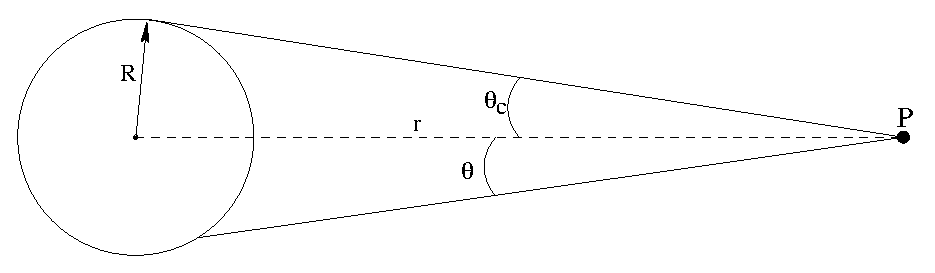
\includegraphics[width=12cm]{figs/bright_sphere}
  \caption{Flux from a uniformly bright sphere.
  \label{fig:bright_sphere}}
\end{figure*}
%%%%%%%%%%%%%%%%%%%%%%%%%%%%%%%%%%%%%%%%%%%%%%%%%%%%%%


Let's look at the relation between the flux and the intensity emitted by a sphere of radius $R$ whose surface emits the same intensity \Inu\ in all directions. This can be considered as a simple model of light emitted by a star. 

Imagine we are in a point $P$ at a distance $r$ from the centre of the sphere (see Fig.~\ref{fig:bright_sphere}). The intensity along rays through $P$ is \Inu\ if the ray intersects the sphere, and zero otherwise. The intensity is non-zero for all angles $\theta \leq \theta_\mathrm{c}$, with 
\be
\sin \theta_\mathrm{c} = \frac{R}{r}.
\ee
For symmetry reasons, the flux at $P$  must be directed radially outward from the sphere, and is given by
\bea
F_\nu &=& \int_0^{2\pi} \int_0^{\theta_\mathrm{c}} \Inu \cos \theta \sin \theta \, \dd \theta\, \dd \phi \nonumber \\ 
  & = & \pi \Inu \sin^2 \theta_\mathrm{c} \nonumber \\ 
  & = & \pi \Inu \left( \frac{R}{r} \right)^2
\eea
This is the familiar inverse square law: the flux from an isotropic source decreases with the square of the distance. We can also compute the total luminosity of the sphere by integrating the flux over the surface of the sphere with radius $r$:
\be
L  = 4 \pi r^2 \cdot \pi \Inu \left( \frac{R}{r} \right)^2 = 4 \pi^2 R^2 \Inu. \label{eq:sphere_lum}
\ee
As expected, the total luminosity of the sphere is independent of $r$. Also note that the flux at the surface of the sphere $r=R$ is simply
\be
F_\nu = \pi \Inu.\label{eq:flux_i}
\ee
Combining Eqs.~\ref{eq:sphere_lum} and \ref{eq:flux_i} yields a relation between luminosity and flux that you might be familiar with from your classes on stellar evolution:
\be
L = 4 \pi R^2 F_\nu,
\ee
which means that the luminosity is simply the product of the surface area of the star times the surface flux.

%%%%%%%%%%%%%%%%%%%%%%%%%%%%%%%%%%%%%%%%%%%%%%%%%%%%%%
\subsection{Resolved and unresolved sources}

%%%%%%%%%%%%%%%%%%%%%%%%%%%%%%%%%%%%%%%%%%%%%%%%%%%%%%
\begin{figure*}
  \centering
  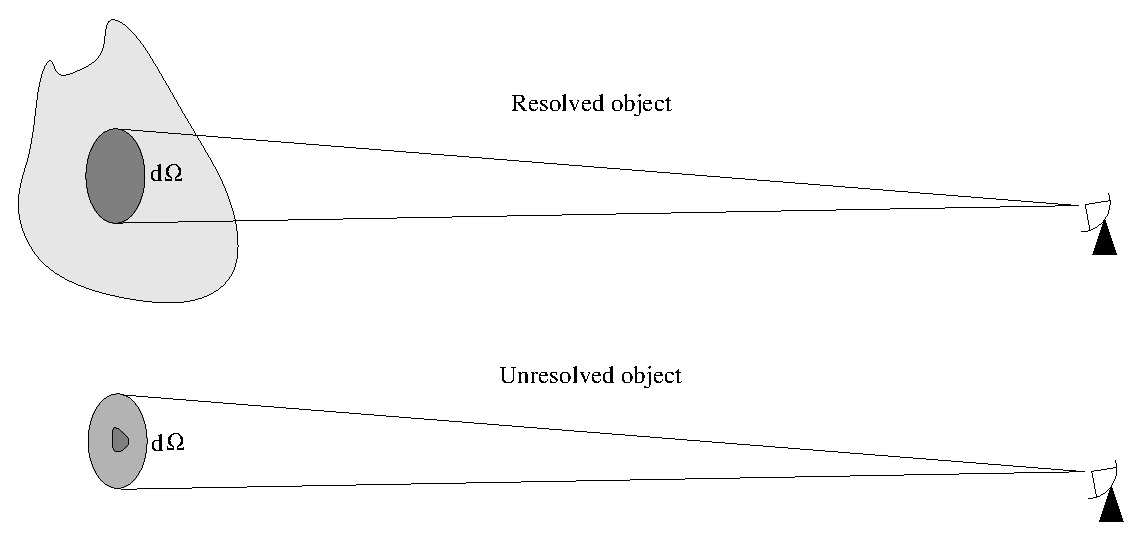
\includegraphics[width=12cm]{figs/resolved_unresolved}
  \caption{Resolved and unresolved sources
  \label{fig:resolved_unresolved}}
\end{figure*}
%%%%%%%%%%%%%%%%%%%%%%%%%%%%%%%%%%%%%%%%%%%%%%%%%%%%%%

A resolution element in a telescope detector (for example a CCD pixel) measures the flux from a beam, by which we mean a constrained part of the sky with solid angle \dO. If \dO\ is small, this flux is proportional to the intensity averaged over \dO. If an astronomical object is resolved, it fills the resolution element completely and only measures the average intensity released in the source, which is also called surface brightness. The flux measured by the resolution element is then independent of the distance to the object. If the object is unresolved, which means its solid angle covers only a fraction of \dO, then one only measures the flux emitted by the object, which does depend on the distance! In radio astronomy one sometimes refers to beam dilution, which is the fraction of the intensity of the source to the beam-averaged intensity.

%%%%%%%%%%%%%%%%%%%%%%%%%%%%%%%%%%%%%%%%%%%%%%%%%%%%%%
\subsection{Magnitudes and Fluxes}
%%%%%%%%%%%%%%%%%%%%%%%%%%%%%%%%%%%%%%%%%%%%%%%%%%%%%%

%%%%%%%%%%%%%%%%%%%%%%%%%%%%%%%%%%%%%%%%%%%%%%%%%%%%%%
\begin{figure*}
\centering
     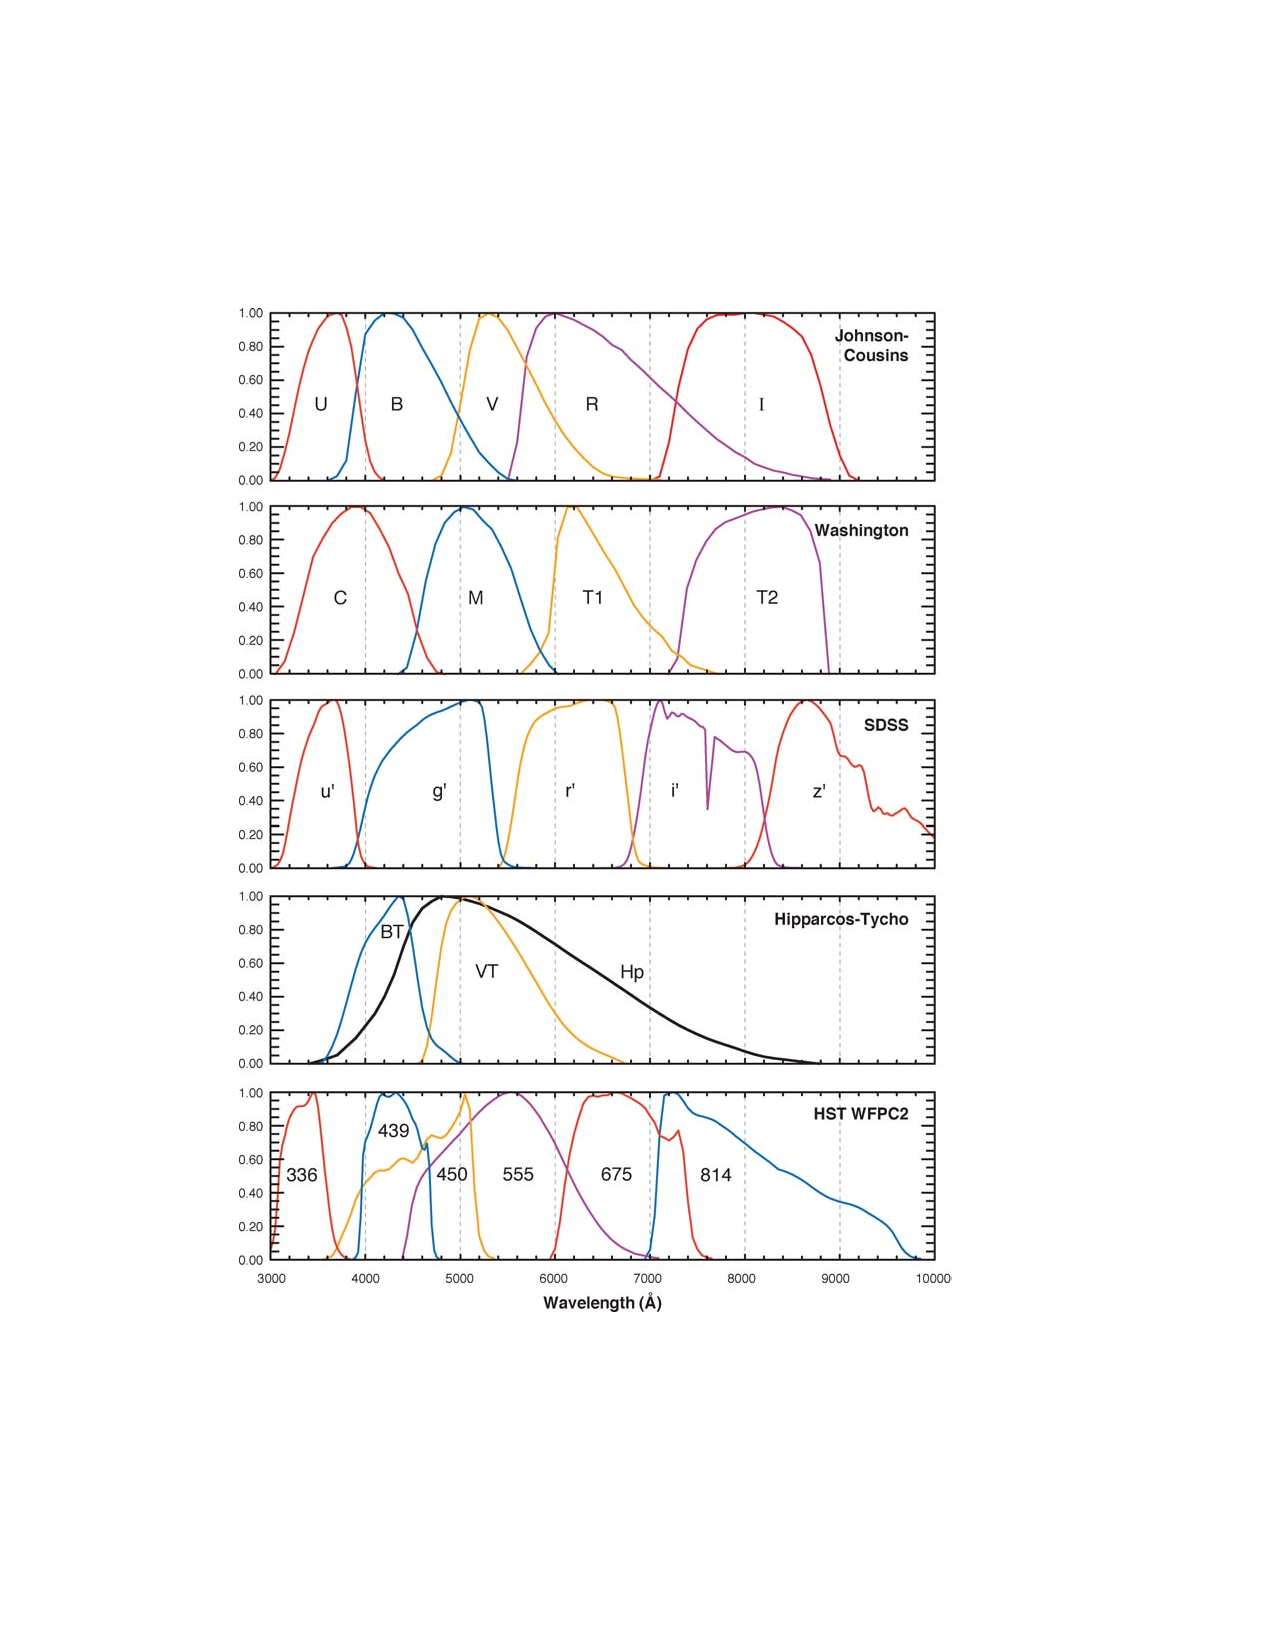
\includegraphics[width=12cm]{figs/photometric_bands}
    \caption{Photometric bands. The colored curves give the sensitivity $S_\lambda$ for different photometry systems and instruments. Figure copied from \citet{2005ARA&A..43..293B}.
     \label{fig:photometric_bands}}
\end{figure*}
%%%%%%%%%%%%%%%%%%%%%%%%%%%%%%%%%%%%%%%%%%%%%%%%%%%%%%

For historical reasons, flux in astronomy has been measured in magnitudes, which are defined as flux ratios:
\be
\mA - \mB = -2.5 \logten \left( \frac{\FA}{\FB} \right),
\ee
where $F_\mathrm{x}$ and $m_\mathrm{x}$ are the flux  and magnitude of object x respectively. In principle magnitudes can be monochromatic, but in practice they are defined over standard bandpasses given as a sensitivity $0 \le S_\lambda \le 1$ as a function of wavelength, called a {\it photometric band}. The flux in a photometric band, say the V band, is given by:
\be
\FV = \frac{\int_0^\infty S_\lambda^\mathrm{V} \Fla \dd \lambda}{\int_0^\infty S_\lambda^\mathrm{V} \dd \lambda}
\ee
and the associated magnitude is 
\be
m^\mathrm{V} = -2.5 \logten \FV + \mathrm{constant}.
\ee 

The {\it bolometric magnitude} is defined for the total energy flux:
\be
F^\mathrm{Bol} = \int_0^\infty  \Fla \, \dd \lambda
\ee
and
\be
m^\mathrm{Bol} = -2.5 \logten F^\mathrm{Bol} + \mathrm{constant}.
\ee
Since magnitudes are relative, one has to use calibration sources to convert to physical flux units. Absolute calibration is a complex subject by itself, so often it is ignored by just relating sources to other ``known'' sources.

%%%%%%%%%%%%%%%%%%%%%%%%%%%%%%%%%%%%%%%%%%%%%%%%%%%%%%
\paragraph{``Adding'' magnitudes} 
Because of their definition, arithmetics with magnitudes is a bit involved. Consider a binary star where the magnitude of the components are \mA\ and \mB. What is their total magnitude \mC? From the definition we have $m = -2.5 \logten F + K$, with K a constant, so that $F = 10^{-0.4m} / 10^{-0.4K}$. Since $\FC = \FA + \FB$, we have:
\be
\frac{10^{-0.4\mC}}{10^{-0.4K}} = \frac{ 10^{-0.4\mA} + 10^{-0.4\mB} }{ 10^{-0.4K} } 
\ee
and
\be
\mC =  -2.5 \logten \left( 10^{-0.4\mA} + 10^{-0.4\mB}  \right)
\ee

%%%%%%%%%%%%%%%%%%%%%%%%%%%%%%%%%%%%%%%%%%%%%%%%%%%%%%
\paragraph{Distance dependence}
Consider a star of luminosity $L$ at a distance $d_1$. If another star of the same luminosity is at distance $d_2$, what is the difference in magnitudes between star 1 and 2? Again, we use what we know of fluxes and apply the definition of magnitudes:
\be
F_1 = \frac{L}{4 \pi d_1^2}, \  F_2 = \frac{L}{4 \pi d_2^2},
\ee
and thus
\be \label{eq:distdepmag}
m_1-m_2 = -2.5 \logten \left( \frac{F_1}{F_2} \right) = -2.5 \logten \left( \frac{d_2^2}{d_1^2} \right)  
               = 5 \logten \frac{d_1}{d_2} 
\ee
\paragraph{Flux ratios in magnitudes} 
Again consider a binary at distance $d_1$ with components of magnitude \mA\ and \mB. How does the magnitude difference $\Delta m = \mB -\mA$ change with distance? Using Eq.~\ref{eq:distdepmag} we have
\bea
 \mB(d_2) =\mB(d1) -5 \logten \frac{d_1}{d_2} \nonumber \\
 \mA(d_2) =\mA(d1) -5 \logten \frac{d_1}{d_2} 
\eea
and so
\be
\mB(d_2)-\mA(d_2)= \mB(d_1)-\mA(d_1) = \Delta m.
\ee
The flux ratio $\Delta m$ is thus invariant with distance.

Specific intensity, or surface brightness, can be expressed as mag$/$arcsec$^2$, where an arcsecond is 1/3600 of a degree, and there are ~206,265 arcsec in a radian (which is also the number of astronomical units in a parsec! Is that a coincidence?). The surface brightness measured in mag$/$arcsec$^2$ is also a conserved quantity, therefore extended objects like galaxies and nebulae have in principle a surface brightness that is independent of distance. In practice other effects come into play, such as extinction by interstellar/galactic material and the expansion of the universe at cosmological distances.

%%%%%%%%%%%%%%%%%%%%%%%%%%%%%%%%%%%%%%%%%%%%%%%%%%%%%%
\section{Radiative transfer}
%%%%%%%%%%%%%%%%%%%%%%%%%%%%%%%%%%%%%%%%%%%%%%%%%%%%%%

%%%%%%%%%%%%%%%%%%%%%%%%%%%%%%%%%%%%%%%%%%%%%%%%%%%%%%
\subsection{Definitions}

So far we have only considered radiation in vacuum, without interaction with matter. In vacuum $\dd \Inu / \ds =0 $ along a ray. To model intensity creation and destruction we introduce a number of new macroscopic definitions.

%%%%%%%%%%%%%%%%%%%%%%%%%%%%%%%%%%%%%%%%%%%%%%%%%%%%%%
  \begin{SCfigure*}
   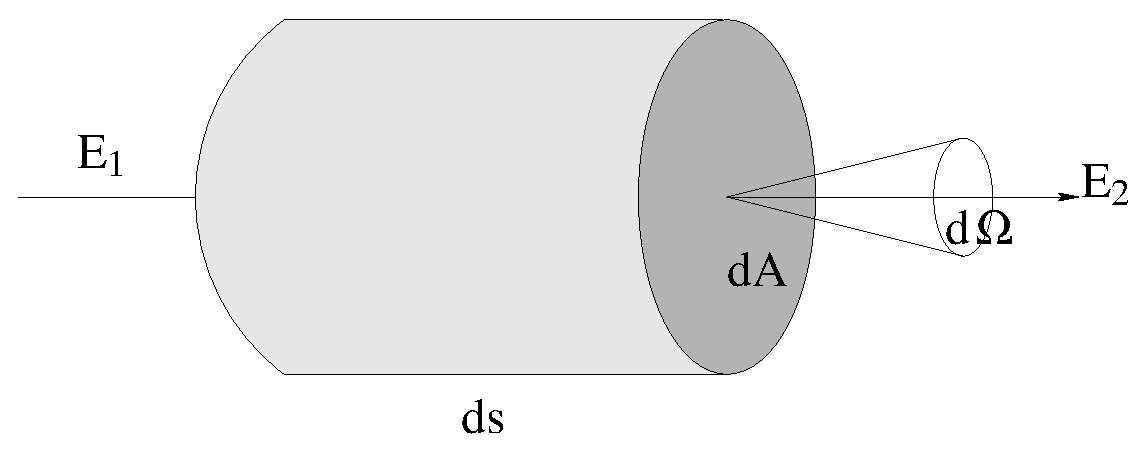
\includegraphics[width=6cm]{figs/emissivity_def}
    \caption{Definition of emissivity. \label{fig:emissivity_def}}
    \end{SCfigure*}
%%%%%%%%%%%%%%%%%%%%%%%%%%%%%%%%%%%%%%%%%%%%%%%%%%%%%%

%%%%%%%%%%%%%%%%%%%%%%%%%%%%%%%%%%%%%%%%%%%%%%%%%%%%%%
\paragraph{Emissivity} 
The monochromatic emissivity \jnu\ is defined as the energy emitted per unit volume per unit time per unit bandwidth and per unit solid angle:
\be
\dd E = \jnu \, \dd V \, \dd t \, \dnu \, \dO.
\ee
It has units of W m$^{-3}$ Hz$^{-1}$ ster$^{-1}$. Imagine a volume $\mathrm{d}V$ with cross section $\mathrm{d}A$ and thickness $\ds$ in which the emissivity is non-zero (see Figure~\ref{fig:emissivity_def}). A beam of radiation enters the volume on the left, and exits it on the right. The emissivity will add energy to the beam. The difference in energy is given by
\bea
E_2 - E_1 & = & \left( I_{\nu,2} - I_{\nu,1} \right)  \dO \, \dnu \, \dt \, \dd A \\
                 & = & \jnu \, \dO \, \dnu \, \dt \, \dd A \, \ds
\eea
Therefore a beam traveling a distance \ds\ though a medium with non-zero emissivity increases its intensity by
\be
\dd \Inu = \jnu \, \ds
\ee

%%%%%%%%%%%%%%%%%%%%%%%%%%%%%%%%%%%%%%%%%%%%%%%%%%%%%%
\paragraph{Extinction} 

%%%%%%%%%%%%%%%%%%%%%%%%%%%%%%%%%%%%%%%%%%%%%%%%%%%%%%
  \begin{SCfigure*}
   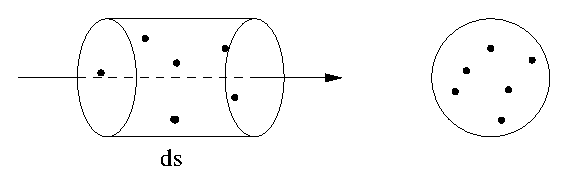
\includegraphics[width=8.8cm]{figs/extinction_def}
    \caption{Left: A beam of cross section $\dd A$ travelling through a region with absorbing particles. Right: view at the region along the beam direction. \label{fig:extinction_def}}
    \end{SCfigure*}
%%%%%%%%%%%%%%%%%%%%%%%%%%%%%%%%%%%%%%%%%%%%%%%%%%%%%%

The monochromatic extinction coefficient is defined as the fraction of energy removed from a beam as it travels a distance $\ds$ through a medium:
\be
\dd \Inu = - \anu \Inu \, \ds.
\ee
The extinction coefficient has units ``per length'', but can also be interpreted as ``area per volume'' (m$^2$ per m$^{-3}$). The latter interpretation follows naturally from a microscopic model of particles, each with an effective cross section $\sigma_\nu$ (see Figure~\ref{fig:extinction_def}). The extinction coefficient is then the fraction of the cross-section of a beam blocked by absorbing particles per unit length. If the particle density is $n$ then $\anu = \sigma_\nu n$.  This view of absorption of radiation is valid only if the particles are distributed at random through the medium, and the ``size'' of the particles $\sigma_\nu^{1/2}$ is much smaller than the mean interparticle distance $n^{-1/3}$. This is usually the case in the outer layers of stars and interstellar material, but not necessarily in the dense interior of stars.

Extinction can also be defined as a cross section per unit mass $\kappa_\nu$.  Then the extinction coefficient becomes $\anu = \kappa_\nu \rho$, with $\rho$ the mass density.

%%%%%%%%%%%%%%%%%%%%%%%%%%%%%%%%%%%%%%%%%%%%%%%%%%%%%%
\subsection{The radiative transfer equation}

If a beam travels through a medium with both emission and extinction then
\be
\dd \Inu = \jnu \, \ds - \anu \, \Inu \, \ds,
\ee
or
\be
\frac{\dd \Inu}{\ds} = \jnu  - \anu \, \Inu.
\ee

%%%%%%%%%%%%%%%%%%%%%%%%%%%%%%%%%%%%%%%%%%%%%%%%%%%%%%
\paragraph{Emissivity only} 
If a medium has zero extinction then the radiative transfer equation reduces to 
\be
\frac{\dd \Inu}{\ds} = \jnu 
\ee
which has the solution
\be
\Inu(s) = \Inu(s_0) + \int_{s_0}^{s} \jnu(s') \, \dd s'.
\ee
In this case the intensity can increase indefinitely as long as the beam travels through the medium.

%%%%%%%%%%%%%%%%%%%%%%%%%%%%%%%%%%%%%%%%%%%%%%%%%%%%%%
\paragraph{Absorption only} 
In the case of $\jnu=0$ we need to solve
\be
\frac{\dd \Inu}{\ds} = - \anu \Inu.
\ee
This equation can be rewritten as
\bea
\frac{1}{\Inu} \frac{\dd \Inu}{\ds} &=& - \anu  \nonumber \\
\frac{\dd  \ln{\Inu} }{\ds} &=&  - \anu \nonumber 
\eea
which can be integrated directly to yield
\be \label{eq:extonly}
\Inu(s) = \Inu(s_0) \, \mathrm{exp} \left(-\int_{s_0}^s \anu(s') \, \dd s'\right).
\ee
The larger the absorption coefficient, the quicker intensity is attenuated as it travels through a medium.

\paragraph{Optical path length} We define the monochromatic optical path length \taunu\ as
\be
\taunu = \int_{s_0}^s \anu(s') \, \dd s'
\ee
This is a dimensionless quantity. An equivalent definition is
\be
\dd \taunu =  \anu\, \ds.
\ee

Let us now consider a slab of material of thickness $D$ between $s=0$ and $s=D$. A beam passes through this slab at a right angle. The total optical path length through the slab is just
\be
\taunu(D) = \int_{0}^s \anu(s) \, \dd s
\ee
One can also say that the slab has a monochromatic optical thickness $\taunu(D)$. It is a measure of how easily photons can penetrate the slab, because Eq.~\ref{eq:extonly} can be written in terms of the optical thickness in a particularly easy form:
\be
\Inu(D) = \Inu(0) \exp^{-\taunu(D)}.
\ee
The intensity decreases exponentially as a function of the optical path length. A slab is called optically thick if $\taunu >1$ and called optically thin if $\taunu <1$.

We can now compute how deep in terms of optical path length a beam can propagate into an object. It is the average optical path length a photon can propagate into the object before it is absorbed. It is given by
\be
<\taunu> = \frac{\int_0^\infty \taunu \exp^{-\taunu} \dd \taunu}{\int_0^\infty \exp^{-\taunu} \dd \taunu} = 1.
\ee
If the object is homogeneous so that $\anu(s)$ is constant we can also compute the mean geometrical path length (length expressed in meters) that a photon travels before it is absorbed by the medium:
\be
l_\nu = \frac{<\taunu>}{\anu} = \frac{1}{\anu}
\ee

%%%%%%%%%%%%%%%%%%%%%%%%%%%%%%%%%%%%%%%%%%%%%%%%%%%%%%
\paragraph{Source function}
The source function \Snu\ is defined as 
\be
\Snu = \frac{\jnu}{\anu}. 
\ee
It has the same units as intensity: $\mathrm{W\ m}^{-2} \ \mathrm{Hz}^{-1} \ \mathrm{ster}^{-1}$. We can use it, together with the definition of optical path length to recast the transport equation into an elegant form:
\bea
\frac{\dd \Inu}{\ds} &=& \jnu  - \anu \, \Inu \nonumber \\
\frac{\dd \Inu}{\anu \ds} &=& \frac{\jnu}{\anu}  -\Inu \nonumber \\
\frac{\dd \Inu}{\dd \taunu} &=& \Snu -\Inu \label{eq:transport-equation}
\eea
The form of the radiative transfer equation given in Eq.~\ref{eq:transport-equation} is often just called the transport equation. It describes the change of intensity per unit optical path length along the beam.

%%%%%%%%%%%%%%%%%%%%%%%%%%%%%%%%%%%%%%%%%%%%%%%%%%%%%%
\subsection{Formal solution of the transport equation}

We will now find the general solution to the transfer equation, which means an expression for \Inu\ as a function of the optical path length \taunu\ given a known source function \Snu\ which is allowed to depend on \taunu.
\bea
\frac{\dd \Inu}{\dd \taunu} &=& \Snu -\Inu, \nonumber \\
\frac{\dd \Inu}{\dd \taunu} +\Inu &=& \Snu,  \nonumber  \\
\left( \frac{\dd \Inu}{\dd \taunu} +\Inu \right) \exp^{\taunu} &=& \Snu \exp^{\taunu},  \nonumber  \\
\frac{\dd \Inu  \exp^{\taunu}}{\dd \taunu}  &=& \Snu \exp^{\taunu}  \nonumber,  \\
\Inu(\taunu)  \exp^{\taunu}  - \Inu(0) &=& \int_0^{\taunu} \Snu(\taunu') \, \exp^{\taunu'}  \, \dd \taunu'.
\eea
As a final step we move $\Inu(0)$ to the right-hand side and divide by $\exp^{\taunu}$ to arrive at the {\it formal solution} of the transport equation:
\be
\Inu(\taunu)  = \Inu(0)  \exp^{-\taunu}  +  \int_0^{\taunu} \Snu(\taunu') \, \exp^{-(\taunu-\taunu')}  \, \dd \taunu'.
\label{eq:formal-solution}
\ee
This is the single most important equation in the theory of radiative transfer. The first term on the right-hand side is the initial intensity attenuated because of the optical path length. The second term is the integral of all local contributions $\Snu(\taunu')$ to the intensity along the beam, also attenuated because of the optical path length between \taunu\ and $\taunu'$.

%%%%%%%%%%%%%%%%%%%%%%%%%%%%%%%%%%%%%%%%%%%%%%%%%%%%%%
\subsection{Radiation from a homogeneous medium}

%%%%%%%%%%%%%%%%%%%%%%%%%%%%%%%%%%%%%%%%%%%%%%%%%%%%%%
\begin{figure*}
  \centering
 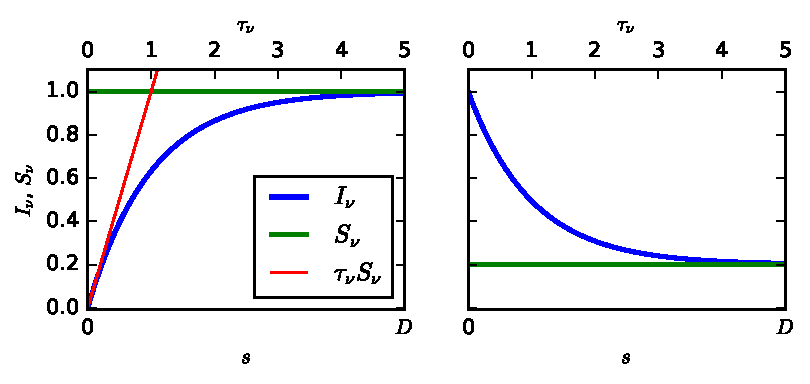
\includegraphics[width=14cm]{figs/homogeneous_slab}
  \caption{Solution to the transfer equation in a homogeneous slab of geometrical thickness $D$ and optical thickness 5. Left-hand panel: $ \Inu(0) = 0$, $\Snu = 1$. The red line shows the linear approximation (Eq.~\ref{eq:linapprox}) valid at small optical depth. Right-hand panel: $ \Inu(0) = 1$, $\Snu = 0.2$.
  \label{fig:homogeneous_slab}}
\end{figure*}
%%%%%%%%%%%%%%%%%%%%%%%%%%%%%%%%%%%%%%%%%%%%%%%%%%%%%%

%%%%%%%%%%%%%%%%%%%%%%%%%%%%%%%%%%%%%%%%%%%%%%%%%%%%%%
\begin{figure*}
  \centering
 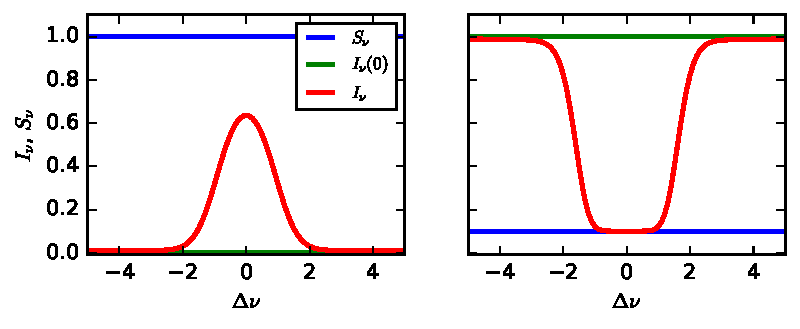
\includegraphics[width=14cm]{figs/homogeneous_slab_spectrum}
  \caption{Solution to the transfer equation in a slab with constant source function, but a frequency-dependent opacity. The blue line shows the source function in the slab, the green line the incoming intensity and the red curve the outgoing intensity. Left-hand panel: $ \Inu(0) = 0$, $\Snu = 1$, $\tau_{\Delta \nu=5} = 0.01$, and $\tau_{\Delta \nu=0} = 1.01$ . Right-hand panel: $ \Inu(0) = 1$, $\Snu = 0.1$, $\tau_{\Delta \nu=5} = 0.01$, and $\tau_{\Delta \nu=0} = 10.01$. \label{fig:homogeneous_slab_freq}}
\end{figure*}
%%%%%%%%%%%%%%%%%%%%%%%%%%%%%%%%%%%%%%%%%%%%%%%%%%%%%%


Let's look at the radiation in a homogenous layer to get some feeling for the behaviour of the formal solution. Again we consider a layer of geometrical thickness $D$ and constant \jnu\ and \anu\ throughout the layer, so that \Snu\ is also constant in the layer and the optical thickness $\taunu = \anu D$. The formal solution for radiation exiting this layer then reduces to
\be
\Inu(\taunu)  = \Inu(0) \, \exp^{-\taunu}  +  \Snu \, (1-\exp^{-\taunu}). \label{eq:homogeneous_slab}
\ee 
If the layer is very optically thick ($\taunu \gg 1$), then 
\be
\Inu(\taunu) \approx  \Snu.
\ee 
Incident radiation cannot penetrate the layer and one receives an intensity equal to the source function.
If the layer is optically thin ($\taunu \ll 1$) then
\be
\Inu(\taunu)  = \Inu(0) +  \taunu \left(  \Snu -\Inu(0) \right), \label{eq:linapprox}
\ee
which means that incident radiation travels mostly straight through the layer, with a slight modification owing to absorption and emission. In general, if $\Snu > \Inu(0)$ then energy (or equivalently: photons) is added to the beam as it propagates; if $\Snu < \Inu(0)$ energy is removed from the beam. Figure~\ref{fig:homogeneous_slab} shows solutions to Eq.~\ref{eq:homogeneous_slab} for two different cases.

So far we have looked at the behaviour of the intensity at a single frequency. We are often also interested in the variation of intensity with frequency, i.e., the shape of the spectrum. As an initial example we can look at a homogeneous slab with a source function that is independent  of frequency, but an extinction coefficient that varies with frequency. Figure~\ref{fig:homogeneous_slab_freq} shows two examples where the extinction coefficient varies as a so-called {\em Voigt function} (for now it's sufficient to know that this is a sharply-peaked function, in Section~\ref{subsec:combining_broadening} the details are given). As you can see it is possible for such a slab to generate an emission line, or an absorption line, depending on the values of $\Snu$ and $\Inu(0)$. Also note that the absorption line has a very flat core, even though the extinction coefficient is sharply-peaked in frequency. This is because Eq.~\ref{eq:homogeneous_slab} implies $\Inu(\taunu)  \approx  \Snu$ for the substantial frequency interval around $\Delta \nu = 0$ where $\taunu \gg 1$.
%%%%%%%%%%%%%%%%%%%%%%%%%%%%%%%%%%%%%%%%%%%%%%%%%%%%%%
\subsection{Radiation from an optically thick medium}

%%%%%%%%%%%%%%%%%%%%%%%%%%%%%%%%%%%%%%%%%%%%%%%%%%%%%%
\begin{figure*}
  \centering
  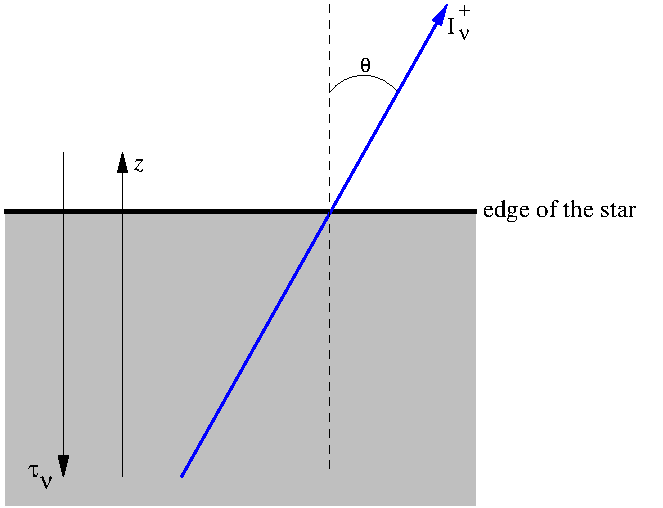
\includegraphics[width=8.8cm]{figs/plane_parallel}
  \caption{Geometry of the plane-parallel stellar atmosphere. The height coordinate $z$ increases outwards from the star, while the optical depth coordinate $\taunu$ increases inward. The angle between the ray and the vertical is $\theta$, with $\mu = \cos{\theta}$.}
\end{figure*}
%%%%%%%%%%%%%%%%%%%%%%%%%%%%%%%%%%%%%%%%%%%%%%%%%%%%%%


The assumption of a homogenous medium is not very realistic. In most cases the absorption coefficient and emissivity depend on the location in the medium. We will now relax the assumption of homogeneity and allow for variation along one direction, say along the $z$ axis. If the medium is in addition optically thick at all frequencies (one cannot look through it) then one has a simple model to describe the atmosphere of a star, called a {\it plane parallel atmosphere}. We assume that the atmosphere has finite extent, so that $\anu=0$ and  and $\jnu=0$ for $z>z_\mathrm{max}$. For outside observers looking at such an atmosphere it is natural to wonder from {\it how deep} in the atmosphere the photons that we see originate. To facilitate this we define a quantity that measures ``deepness'' in the atmosphere, called radial optical depth $\taunu'$. It is defined so that for a location $z$ inside the atmosphere: 
\be
\taunu'(z) = -\int_\infty^z \anu(z') \, \dd z'
\ee
It is very similar to the optical path length, except that we integrate against the propagation direction of the beam, instead of along it: $\dd \taunu' = - \anu \, \ds$, whereas $\dd \taunu = \anu \, \ds$. To facilitate ease of notation we will drop the prime on the optical depth and use $\taunu$ for both radial optical depth as optical thickness. Which quantity is meant is (hopefully) clear from the context.

For rays that are not parallel to the $z$-axis, but instead have an angle $\theta$ with the $z$-axis, with $\mu = \cos{\theta}$ we can define an angle-dependent optical depth $\taumunu$:
\be
\dd \taumunu = \frac{\dd \taunu}{\cos \theta} = \frac{\dd \taunu}{\mu}.
\ee
The transport equation then becomes
%\be
%\mu \frac{\dd \Inu}{\dd \tau_\nu} = \Inu - \Snu.
%\ee 
\be
\mu \frac{\dd \Inu(\taunu,\mu)}{\dd \tau_\nu} = \Inu(\taunu,\mu) - \Snu(\taunu),
\ee 
where the dependency of $\Inu$ means ``at the radial optical depth $\taunu$ and in the direction $\mu$'' and the dependency of $\Snu$ means that it depends only on radial optical depth but not on direction.

Now imagine you are sitting at a radial optical depth $\taunu$ inside the atmosphere. What is the inward intensity at that point. Rays traveling into the star have $\mu<0$, so we can write the formal solution as 
\be
\Inu^-(\taunu,\mu)  =  - \int_0^{\taunu} \Snu(t_\nu) \, \exp^{-(t_\nu-\taunu)/\mu} \frac{\dd t_\nu}{\mu}.
\ee
For outgoing rays ($\mu>0$) the formal solution is
\be
\Inu^+(\taunu,\mu)  =   \int_{\taunu}^{\infty} \Snu(t_\nu) \, \exp^{-(t_\nu-\taunu)/\mu} \frac{\dd t_\nu}{\mu}.
\ee
For an observer outside of the atmosphere (so at $\taunu=0$) and for an angle $\mu>0$ this expression simplifies to
\be
 \label{eq:escrad}
\Inu^+(0,\mu)  =   \int_0^{\infty} \Snu(t_\nu) \, \exp^{-t_\nu/\mu} \frac{\dd t_\nu}{\mu}. 
\ee
In words, this equation means that the intensity escaping from a stellar atmosphere (or any optically thick object) is set by the source function from the top of the atmosphere (optical depth $\taunu=0$) to an optical depth where the exponential drives the integrand to zero (say $\taunu=10$ or so.).

%%%%%%%%%%%%%%%%%%%%%%%%%%%%%%%%%%%%%%%%%%%%%%%%%%%%%%
\begin{figure*}
  \centering
  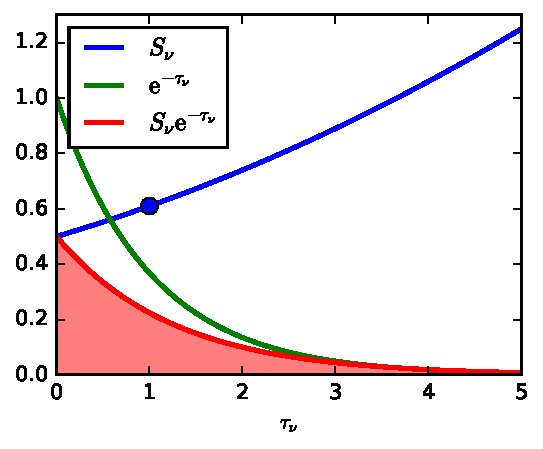
\includegraphics[width=8.8cm]{figs/eddington_barbier}
  \caption{The Eddington Barbier approximation for $\mu=1$  \label{fig:EB}. The surface of the colored area under the red curve is approximately equal to the source function at $\taunu=1$ (indicated with the blue filled circle).}
\end{figure*}
%%%%%%%%%%%%%%%%%%%%%%%%%%%%%%%%%%%%%%%%%%%%%%%%%%%%%%

At what height does the radiation typically escape? We can compute this by substituting a series expansion of the source function into Eq.~\ref{eq:escrad}. So we assume
\be
  \Snu(\taunu) = \sum_{n=0}^\infty a_n \, \taunu^n,
\ee
and use the mathematical identity
\be
\int_0^\infty = x^n \exp^{-x} \dd x = n!
\ee
to find
\be
\Inu^+(\taunu=0,\mu) = a_0 + a_1 \mu + 2 a_2 \mu^2 + \cdots.
\ee 
If we truncate the expansion after the first two terms we get the {\it Eddington-Barbier} approximation
\be
\Inu^+(\taunu=0,\mu) \approx \Snu(\taunu=\mu).
\ee 
In words this approximation states that if one observes a stellar atmosphere under a viewing angle $\mu$, then one sees an intensity that is approximately equal to the source function at radial optical depth $\taunu=\mu$.

%%%%%%%%%%%%%%%%%%%%%%%%%%%%%%%%%%%%%%%%%%%%%%%%%%%%%%
\section{Radiation in thermodynamic equilibrium}
%%%%%%%%%%%%%%%%%%%%%%%%%%%%%%%%%%%%%%%%%%%%%%%%%%%%%%

%%%%%%%%%%%%%%%%%%%%%%%%%%%%%%%%%%%%%%%%%%%%%%%%%%%%%%
\subsection{Black-body radiation}
%%%%%%%%%%%%%%%%%%%%%%%%%%%%%%%%%%%%%%%%%%%%%%%%%%%%%%

%%%%%%%%%%%%%%%%%%%%%%%%%%%%%%%%%%%%%%%%%%%%%%%%%%%%%%
\begin{figure*}
  \centering
  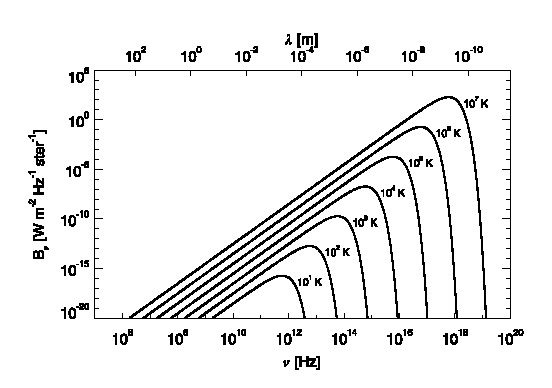
\includegraphics[width=8.8cm]{figs/Bnu}
  \caption{The Planck function per frequency interval for different temperatures.
  \label{fig:Bnu_def}}
\end{figure*}
%%%%%%%%%%%%%%%%%%%%%%%%%%%%%%%%%%%%%%%%%%%%%%%%%%%%%%

A perfect black body emits radiation with an intensity equal to to the Planck function \Bnu:
\be
\Bnu = \Plancknu.
\ee
The Planck function has the same units as intensity, and in terms of wavelength intervals it is given by:
\be
\Bla = \Bnu \left| \frac{\dd \nu}{\dd \lambda} \right| = \Planckla.
\ee
For large values of $h \nu / kT$ the {\it Wien approximation} is sometimes used:
\be
\Bnu \approx \frac{2 h \nu^3}{c^2} \exp^{-h \nu / kT}.
\ee
If $h \nu / kT \ll 1$ then the more common  {\it Rayleigh-Jeans approximation}  is used:
\be
\Bnu \approx \frac{2 h \nu^2 k T}{c^2}.
\ee
Note that the derivative of the Planck law with respect to temperature is always positive.

%%%%%%%%%%%%%%%%%%%%%%%%%%%%%%%%%%%%%%%%%%%%%%%%%%%%%%
\paragraph{Wien displacement law} 
The Wien displacement law gives the frequency $\nu_\mathrm{max}$ where the Planck function peaks, i.e, where
\be
\frac{\partial \Bnu}{\partial \nu} = 0.
\ee
This equation cannot be solved analytically, but has the approximate solution:
\be
\frac{\nu_\mathrm{max}}{T} = 5.88 \times 10^{10} \ \mathrm{Hz}\ \mathrm{K}^{-1}
\ee
If the Planck function is expressed per wavelength unit to find $\lambda_\mathrm{max}$ where 
\be
\frac{\partial \Bla}{\partial \lambda} = 0.
\ee
then
\be
\lambda_\mathrm{max} T = 2.90 \times 10^{-3} \ \mathrm{m}\ \mathrm{K}^{-1}.
\ee
Note that 
\be
\lambda_\mathrm{max} \ne \frac{c}{\nu_\mathrm{max} }
\ee

%%%%%%%%%%%%%%%%%%%%%%%%%%%%%%%%%%%%%%%%%%%%%%%%%%%%%%
\paragraph{Stefan-Boltzmann}
Integrating the Planck function over the whole spectrum gives the {\it Stefan-Boltzmann law}.
\be
B=\int_0^\infty \Bnu \, \dd \nu = \frac{\sigma}{\pi} T^4
\ee
with
\be
\sigma= \frac{2 \pi^5 k^4}{15 h^3 c^2} = 5.67 \times 10^{-8} \ \mathrm{W}\ \mathrm{m}^{-2} \mathrm{K}^{-4}.
\ee
The total flux radiated by the surface of a black body is therefore $\pi I = \sigma T^4$.

Even if \Fnu\ is not well approximated by flux from a black body, the Stefan-Boltzmann law can always be used to define an {\it effective temperature}:
\be
T_\mathrm{eff} = \left( \frac{F}{\sigma} \right)^{1/4}
\ee
Similarly, one can define a {\it brightness temperature} or {\it radiation temperature} $\Tb(\nu)$ such that 
\be
\Inu = \Bnu(\Tb).
\ee
Since \Bnu\ is a monotonous function of $T$, this relation can be used to express any intensity in units of temperature. This is used in particular in radio astronomy, where the Rayleigh-Jeans approximation is often applicable. A motivation for doing this is that the brightness temperature is often related to physical properties of the emitter, and has a simple unit (K).

%%%%%%%%%%%%%%%%%%%%%%%%%%%%%%%%%%%%%%%%%%%%%%%%%%%%%%
\subsection{Transfer equation and source function in thermodynamic equilibrium}
%%%%%%%%%%%%%%%%%%%%%%%%%%%%%%%%%%%%%%%%%%%%%%%%%%%%%%

In order to make the coupling of the macroscopic quantities \anu, \jnu\ and \Snu\ to properties of microscopic quantum-mechanical systems (atoms or molecules for example), we need to investigate the properties of radiation in a homogeneous medium in thermodynamic equilibrium (TE). In TE all processes and states are in equilibrium with each other. Each process is in equilibrium with the reverse process. This is called detailed balance. As a model system you can imagine an oven with perfect blackbody walls at a temperature $T$ filled with some material.

The radiation inside the material must be static in time and isotropic. Therefore, for any ray, at any frequency, and any time the following must hold:
\be
\frac{\dd \Inu}{\dd s} = \jnu -\anu \Inu = 0,
\ee
and therefore
\be
 \jnu = \anu \Inu.
\ee 
But we know from  thermodynamic theory that the radiation in TE follows the Planck function:
\be
{\Inu}_\mathrm{,TE} =\Bnu,
\ee
and therefore the source function is also the Planck function in TE:
\be
{\Snu}_\mathrm{,TE} =\frac{\jnu}{\anu}=\Bnu,
\ee

%%%%%%%%%%%%%%%%%%%%%%%%%%%%%%%%%%%%%%%%%%%%%%%%%%%%%%
\section{Matter in thermodynamic equilibrium}
%%%%%%%%%%%%%%%%%%%%%%%%%%%%%%%%%%%%%%%%%%%%%%%%%%%%%%

%%%%%%%%%%%%%%%%%%%%%%%%%%%%%%%%%%%%%%%%%%%%%%%%%%%%%%
\paragraph{Maxwell distribution}

If the kinetic energy of particles in a gas is in thermodynamic equilibrium it follows the Maxwellian velocity distribution. The probability that a particle of mass $m$ has velocity component $v_x$ between $v_x$ and $v_x+\dd v_x$ is given by
\be
P(v_x) \, \dd v_x = \left( \frac{m}{2\pi kT}  \right)^{1/2} \,  \exp^{-(1/2) m v_x^2 / kT }  \dd v_x
\ee
For the speed $v$ the probability is
\be
P(v) \, \dd v = \left( \frac{m}{2\pi kT}  \right)^{3/2} 4\pi v^2 \, \exp^{-(1/2) m v^2 / kT }  \dd v.
\ee
In stellar atmospheres and the interstellar medium this relation is usually true also outside of TE.

%%%%%%%%%%%%%%%%%%%%%%%%%%%%%%%%%%%%%%%%%%%%%%%%%%%%%%
\paragraph{Boltzmann distribution}
In TE, the  ratio of particle population between 2 discrete energy levels $i$ and $j$ in a quantum-mechanical system, like a specific atom or molecule is given by the Boltzmann law:
\be
\frac{n_i}{n_j} = \frac{g_i}{g_j} \, \exp^{-(\chi_i- \chi_j)/kT}.
\ee
Here $\chi_i$ is the energy of the bound level $i$. Normally the ground state of an atom is defined to have $\chi=0$.
The fraction of all atoms in a given ionization state in level $i$ is given by
\be
\frac{n_i}{N} = \frac{g_i}{U} \, \exp^{-\chi_i/kT},
\ee
with $N$ the total density of the particles in any state and $U$ the partition function.

%%%%%%%%%%%%%%%%%%%%%%%%%%%%%%%%%%%%%%%%%%%%%%%%%%%%%%
\paragraph{Saha distribution}
Atoms and molecules can exist in different ionisation stages. At higher temperatures the higher ionisation stage is typically more populated. The ratio of densities of an atomic species in ionization stage $r$ and $r+1$ is given by the Saha distribution:
\be
\frac{N_{r+1}}{N_r} = \frac{1}{\nelec} \frac{2 U_{r+1}}{U_r}  \left( \frac{2 \pi m_\mathrm{e} k T}{h^2} \right)^{3/2}  \exp^{-(\chi_r)/kT}.
\ee
For molecules a very similar formula holds.

%%%%%%%%%%%%%%%%%%%%%%%%%%%%%%%%%%%%%%%%%%%%%%%%%%%%%%
\paragraph{Saha-Boltzmann}
The Saha and Boltzmann law combined give all information needed to compute the relative populations in any energy level of any species of an arbitrary gas mixture. In order to get absolute populations (number of particles in a given quantum state per unit volume), the two laws must be augmented with two extra laws: The first one is element conservation, i.e, the total number density of nuclei of an element is conserved:
\be
\sum_r \sum_i N_{r,i} = N_\mathrm{element},
\ee
where the sum is over all ionization stages $r$ and all energy levels $i$ in the ionisation state $r$. In addition we need a charge conservation equation, because the Saha equation contains the electron density:
\be
\sum_\mathrm{element} \sum_r Z_r N_r= \nelec,
\ee
where $Z_r$ is the charge of ionisation stage $r$. These equations must in general be solved numerically, for example with Newton-Raphson iteration. This might seem a bit off-topic here, but it is an important ingredient of understanding radiative transfer. If TE is a good approximation, then the gas density, temperature and the elemental composition (abundances) set all particle densities, and, as a consequence the extinction coefficients. The source function is the Planck function. These assumptions underpin a large part of stellar modelling and the modelling of stellar atmospheres.

%%%%%%%%%%%%%%%%%%%%%%%%%%%%%%%%%%%%%%%%%%%%%%%%%%%%%%
\section{Matter/radiation interaction}
%%%%%%%%%%%%%%%%%%%%%%%%%%%%%%%%%%%%%%%%%%%%%%%%%%%%%%

Individual particles of matter have internal (bound) energy states which are discrete (quantised), which we often denote by $E_n$. Interaction between unbound (``free'') particles have a continuous distribution of possible energy states. A system switches energy state by interaction with either another system (collision) or photons (emission/absorption). A radiative transition between two states $E_u$ and $E_l$  with $E_u>E_l$ causes a photon of energy 
\be
h \nu = E_u-E_l
\ee
to be emitted or absorbed.

We usually distinguish between three types of energy state transitions: bound-bound, free-free and bound-free. A bound-free transition involves a system splitting into two, or two systems combining into one. Typical examples are the ionisation of an atom into an ion-electron pair, or the break-up of a molecule into smaller molecules and/or atoms (dissoc
ation).

%%%%%%%%%%%%%%%%%%%%%%%%%%%%%%%%%%%%%%%%%%%%%%%%%%%%%%
\subsection{Bound-bound transitions}

There are five processes that cause a transition from one bound state to another
\begin{itemize}
\item spontaneous radiative deexcitation
\item radiative excitation
\item induced radiative deexcitation
\item collisional deexcitation
\item collisional excitation
\end{itemize}

%%%%%%%%%%%%%%%%%%%%%%%%%%%%%%%%%%%%%%%%%%%%%%%%%%%%%%
\paragraph{Spontaneous  deexcitation}
A particle in upper level $u$ can decay spontaneously to a lower energy level $l$, while emitting a photon. The probability that this will occur is defined as the {\it Einstein coefficient} $A_{ul}$: the transition probability for spontaneous deexcitation per second per particle in state $u$. The population level $u$ over time is given as
\be
n_u(t) = n_u(0) \exp^{-A_{ul}t}.
\ee
Heisenberg's uncertainty principle states that because of the finite lifetime of the upper level, there is a uncertainty about the energy of the level:
\be
\Delta E \approx \frac{h}{2 \pi \Delta t}.
\ee
The energy of the emitted photon thus exhibits a certain spread around the value $E_u-E_l$. A proper quantum-mechanical treatment gives a Lorentzian distribution for the photon energy around the line frequency $\nu_0$:
\be
\psi(\nu-\nu_0) = \frac{A_{ul}/ 4 \pi^2}{(\nu-\nu_0)^2 + (A_{ul}/4 \pi)^2}
\ee
This is the profile function for spontaneous deexcitation of an atom at rest. It is normalised with respect to frequency and has units Hz$^{-1}$.

%%%%%%%%%%%%%%%%%%%%%%%%%%%%%%%%%%%%%%%%%%%%%%%%%%%%%%
\paragraph{Radiative excitation} A photon with the right energy $h\nu$ can excite a system from state $l$ to state $u$. The probability that this happens is given by:
\be
B_{lu} \Jbar^\phi,
\ee
which is the number of radiative excitations per second per particle in state $l$. The energy states have a certain fuzziness, and therefore one needs to account for the spread in photon energy:
\be
\Jbar^\phi = \int_0^\infty \Jnu \, \phi (\nu-\nu_0) \dd \nu.
\ee
The quantity $\phi (\nu-\nu_0)$ is the normalised profile function for spontaneous excitation.

%%%%%%%%%%%%%%%%%%%%%%%%%%%%%%%%%%%%%%%%%%%%%%%%%%%%%%
\paragraph{Induced deexcitation}
It turns out there is a process that causes a transition from state $u$ to $l$ in the presence of a photon, called induced deexcitation. The transition causes an extra photon to be emitted in the same direction as the first photon. The number of induced deexcitations per second per particle in state $u$ is given by:
\be
B_{ul} \Jbar^\chi,
\ee
where 
\be
 \Jbar^\chi = \int_0^\infty \Jnu \, \chi (\nu-\nu_0) \dd \nu.
\ee
Here $\chi(\nu-\nu_0)$ is the normalised profile function for induced deexcitation.

%%%%%%%%%%%%%%%%%%%%%%%%%%%%%%%%%%%%%%%%%%%%%%%%%%%%%%
\paragraph{Collisional excitation and deexcitation}

The transition probability for collisional processes can be defined with similar coefficients $C_{ul}$, the number of collisional deexcitations per second per particle in state $u$. $C_{lu}$ has a similar definition.

These coefficients depend on the type of the colliding particles and their speed. For collisions with electrons we have
\be
C_{lu} = \nelec \int_{v0}^\infty \sigma_{lu}(v) \, v \, f(v) \, \dd v,
\ee 
with $v_0$ the threshold velocity for which $1/2 m_\mathrm{e} v^2 = h\nu_0$,$f(v)$ is usually the Maxwell distribution and $\sigma_{ij}$ a cross section. Note the dependency on the velocity. The cross sections can  in principle be measured in the laboratory, or computed from quantum mechanics. For many transitions they are not well known.  Note the velocity dependence of $C_{ij}$. Light particles move faster than heavy particles, and collide more frequently. For gases where the electron density is similar to the ion density, electron collisions usually dominate. For gases that are nearly neutral, collisions with hydrogen are typically dominant.

%%%%%%%%%%%%%%%%%%%%%%%%%%%%%%%%%%%%%%%%%%%%%%%%%%%%%%
\subsection{Einstein relations}

It turns out that there are relations between $A_{ul}$, $B_{ul}$ and $B_{lu}$. To see this we consider a two-level atom in thermodynamic equilibrium. The number of radiative transitions from $l$ to $u$ must be equal to the number of radiative transitions from $u$ to $l$. If this was not the case then there would be energy exchange between the particles and the radiation field, which cannot happen in TE. Based on quantum mechanics one can also prove that all profile functions are equal ($\psi=\phi=\chi$) and thus $\Jbar = \Jbar^\chi = \Jbar^\phi$. Therefore we can write
\bea
n_l B_{lu} \Jbar^\chi  &= & n_u A_{ul} + n_u B_{ul} \Jbar^\phi \nonumber \\
\Jbar &=& \frac{n_u A_{ul} }{n_l B_{lu} -n_u B_{ul}}   \nonumber \\
   & = & \frac{A_{ul}/B_{ul} }{\dfrac{n_l}{n_u} \dfrac{B_{lu}}{B_{ul}} - 1}.
\eea
Then we use the fact that the Boltzmann distribution holds in TE to get
\be
\Jbar =  \frac{A_{ul}/B_{ul} }{\dfrac{g_l}{g_u} \dfrac{B_{lu}}{B_{ul}} \exp^{h\nu /kT}- 1}.
\ee
In  TE we also know that $\Inu = \Jnu = \Bnu$, and if the profile functions are narrow, then $\Jbar = \Bnu$ as well, so
\be
\Bnu =  \frac{A_{ul}/B_{ul} }{\dfrac{g_l}{g_u} \dfrac{B_{lu}}{B_{ul}} \exp^{h\nu /kT}- 1}.
\ee
By comparing this expression to the formula for the Planck function we find that:
\bea
\frac{A_{ul}}{B_{ul} } &=& \frac{2 h \nu^3}{c^2} \\
\frac{B_{lu}}{B_{ul}} &=& \frac{g_u}{g_l}
\eea
These two equations are the Einstein relations. Note that they only depend on the atomic parameters, they are thus intrinsic properties of the atom and generally valid. If one coefficient is known, either through measurement or calculation, then the other two can be computed.
The strength of a transition is normally reported as an oscillator strength $f_{lu}$:
\be
\frac{4 \pi}{h \nu} B_{lu} = \frac{ \pi e^2}{m_\mathrm{e} c} f_{lu}.
\ee
For strong lines $f_{lu}$ is of order unity. For other allowed (dipole) transitions it lies between $10^{-4}$ and $10^{-1}$. For forbidden lines $f_{lu}< 10^{-6}$.

For the collisional rates the same reasoning holds. The atomic level population does not change in time, and there is no exchange of energy between the radiation field and the atom. Therefore the rate from $l$ to $u$ must be equal to the rate from $u$ to $l$:
\be
n_l C_{lu} = n_u C_{ul}.
\ee
By using the Boltzmann relation we can rewrite this expression as
\be
\frac{C_{ul}}{C_{lu}} = \frac{g_u}{g_l} \exp^{(E_u-E_l) / kT}.
\ee


%%%%%%%%%%%%%%%%%%%%%%%%%%%%%%%%%%%%%%%%%%%%%%%%%%%%%%
\subsection{Emissivity and extinction coefficient}

We are now ready to express the macroscopic emissivity and extinction coefficient for bound-bound transitions in microscopic quantities, namely the profile function and the Einstein coefficients.

%%%%%%%%%%%%%%%%%%%%%%%%%%%%%%%%%%%%%%%%%%%%%%%%%%%%%%
\paragraph{Emissivity}
$n_u A_{ul}$ is the number of spontaneous deexcitatons per second per m$^{3}$ \\
$h \nu_0 n_u A_{ul}$ is energy radiated per second per m$^{3}$  \\
$h \nu_0 n_u A_{ul} \psi(\nu-\nu_0)$ is energy radiated per second per m$^{3}$  per Hz \\
$h \nu_0 n_u A_{ul} \psi(\nu-\nu_0) /4\pi$ is energy radiated per second per m$^{3}$  per Hz per steradian \\

The latter is the definition of emissivity, and we have thus arrived at an expression for the emissivity for spontaneous deexcitation:
\be
\jnu^\mathrm{spon} = \frac{h \nu_0}{4\pi} \, n_u  \,A_{ul}  \, \psi(\nu-\nu_0).
\ee

%%%%%%%%%%%%%%%%%%%%%%%%%%%%%%%%%%%%%%%%%%%%%%%%%%%%%%
\paragraph{Extinction coefficient}
The total energy that is removed from the radiation by line excitation in a volume $\dd V$ and a time $\dd t$ is
\bea
\dd E_\nu^\mathrm{tot} &=&  -h \nu_0 \, n_l \, B_{lu}  \Jbar^\phi \, \dd V  \, \dd t    \nonumber \\
 & =&  -h \nu_0 \, n_l \, B_{lu}  \int \Jnu \phi(\nu-\nu_0) \, \dd \nu  \, \dd V  \, \dd t    \nonumber \\
 & =&  -\frac{h \nu_0}{4 \pi} \, n_l \, B_{lu}  \int \int \Inu \phi(\nu-\nu_0) \, \dO \, \dd \nu  \, \dd V  \, \dd t.  
\eea
The energy taken from a bundle with opening angle \dO\ and in a bandwidth $\dd \nu$ is thus
\be
\dd E_\nu^\mathrm{bundle} = - \frac{h \nu_0}{4 \pi} \, n_l \, B_{lu}  \Inu \phi(\nu-\nu_0) \, \dO \, \dd \nu  \, \dd V  \, \dd t.
\ee
Now note that $\dd V = \dd A \, \dd s$, move all differentials to the left side and note that $\dd \Inu = \dd E / ( \dO \, \dd \nu  \, \dd A  \, \dd t)$. Then we find that
\be
\frac{\dd \Inu}{\dd s} = - \frac{h \nu_0}{4 \pi} \, n_l \, B_{lu}  \phi(\nu-\nu_0) \Inu.
\ee
The extinction coefficient associated with line excitation is therefore
\be
\alpha_\nu^\mathrm{exc.} = \frac{h \nu_0}{4 \pi}  \, n_l \, B_{lu} \phi(\nu-\nu_0).
\ee

Induced deexcitation adds photons to a beam, and one would think this would lead to an emissivity. However, induced deexcitation is proportional to the radiation field $\Jbar$, and therefore behaves much like an opacity. It is therefore much more convenient to model induced deexcitation as  negative extinction. Using similar reasoning as for excitation one arrives at an extinction coeffient
\be
\alpha_\nu^\mathrm{ind.} = -\frac{h \nu_0}{4 \pi}  \, n_u \, B_{ul} \chi(\nu-\nu_0).
\ee
The total line extinction coefficient then becomes
\be
\alpha_{\nu}^\mathrm{line} = \frac{h \nu_0}{4 \pi}  \left( n_l \, B_{lu}  \phi(\nu-\nu_0)- n_u \, B_{ul} \chi(\nu-\nu_0) \right).
\ee
This equation can be rewritten in an interesting form:
\be
\alpha_{\nu}^\mathrm{line} = \frac{h \nu_0}{4 \pi} n_l B_{lu}  \phi(\nu-\nu_0) \left( 1 - \frac{n_u B_{ul} \chi(\nu-\nu_0)}{n_l B_{lu}  \phi(\nu-\nu_0)} \right).
\ee
The line extinction coefficient can be seen to consist of the extinction owing to radiative excitation, with a correction factor owing to induced deexcitation. The correction factor is
\be
1 - \frac{n_u \, B_{ul} \chi(\nu-\nu_0)}{n_l B_{lu}  \phi(\nu-\nu_0)}.
\ee
If it becomes negative then the extinction coefficient becomes negative, and the equation
\be
\frac{\dd \Inu}{\dd s} = - \alpha_\nu \Inu
\ee
has a solution with exponentially growing intensity. Such a negative extinction coefficient requires a so-called population inversion: $n_u g_l > n_l g_u$. This is the principle behind lasers, and in an astrophysical context, masers, which are huge amplification of the intensity in transitions with micrometer wavelengths, often transitions in molecules. Note however that population inversion is not possible in a two-level system, at least a third level is required.

%%%%%%%%%%%%%%%%%%%%%%%%%%%%%%%%%%%%%%%%%%%%%%%%%%%%%%
\subsection{Source function}
Finally we arrive at the expression of the two-level line source function:
\bea
 \Snu^\mathrm{line} &=&\frac{j_\nu}{\anu}  \nonumber \\
    &=& \frac{n_u A_{ul} \psi} {n_l \, B_{lu} \phi - n_u \, B_{ul} \chi } \nonumber \\
      &=& \frac{\dfrac{A_{ul}}{B_{ul}} \dfrac{\psi}{\phi}} {\dfrac{n_l}{n_u} \dfrac{B_{lu}}{B_{ul}} -\dfrac{\chi}{\phi} }.
\eea
If we furthermore assume that all the profile functions are equal $\psi=\phi=\chi$, and plug in the Einstein relations, then the line source function becomes:
\be
\Snu^\mathrm{line} = \frac{2 h \nu^3}{c^2} \frac{1}{ \dfrac{g_u n_l}{g_l n_u} -1}.
\ee
In case the population ratio follows the Boltzmann distribution (which can be taken as the definition of Local Thermodynamic Equilibrium) then the line source function reduces to the Planck function:
\be
S^\mathrm{line}_{\nu0,\mathrm{LTE}} = \Bnu.
\ee
Note that the line source function is nearly frequency-independent  because $\nu^3$ is almost constant over the small frequency range where the profile function is non-zero.

%%%%%%%%%%%%%%%%%%%%%%%%%%%%%%%%%%%%%%%%%%%%%%%%%%%%%%
\section{Line broadening}

The profile function of bound-bound transitions is not infinitely sharp, but broadened owing to a number of different processes. We can distinguish the following broadening processes:
\begin{itemize}
\item natural broadening, due to quantum mechanical effects, as you have seen before,
\item collisional broadening, also called pressure broadening, due to perturbation of the emitting particle by other particles.
\item Doppler broadening, due to particles having different velocities along the line of sight, which can be further subdivided into:
\begin{itemize}	
\item thermal broadening because the particles have thermal velocities,
\item turbulent broadening, because of gas flows parallel to the line of sight,
\item broadening owing to systematic motions, such as rotation of stars.
\end{itemize}	
\item Instrumental broadening, because the instruments with which we observe have finite spectral resolution. This is not a true broadening process as it modifies the intensity that we observe in our telescope, and it is not an intrinsic property of the source.
\end{itemize}
Typically multiple processes are acting at the same time. We will first discuss each process individually, and then discuss how to combine various broadening mechanisms to arrive at the final profile function. Note that the profile function described by the extinction and emission profiles $\psi$, $\phi$ and $\chi$ is strictly speaking modified only by natural, collisional and turbulent broadening. The actual line profile (i.e., the variation of intensity with frequency that we observe) is modified by systematic motions and instrumental broadening, and depends on the telescope and instruments that we use.

%%%%%%%%%%%%%%%%%%%%%%%%%%%%%%%%%%%%%%%%%%%%%%%%%%%%%%
\subsection{Broadening processes}
%%%%%%%%%%%%%%%%%%%%%%%%%%%%%%%%%%%%%%%%%%%%%%%%%%%%%%

%%%%%%%%%%%%%%%%%%%%%%%%%%%%%%%%%%%%%%%%%%%%%%%%%%%%%%
\paragraph{Natural  broadening} We have already seen how Heisenberg's uncertainty principle combined with the finite lifetime of the upper level of a transition lead to the Lorentzian profile:
\be
\psi(\nu-\nu_0) = \frac{\gamma / 4 \pi^2}{(\nu-\nu_0)^2 + (\gamma /4 \pi)^2}.
\ee
In case of the two-level atom we simply have $\gamma=A_{ul}$. For atoms with multiple levels we also have to take into account the lifetime of the lower level, and that the lifetime of a level is determined by all transitions out of the level, not only the transition that we are interested in. It turns out one can directly add the Einstein $A$ coefficients to arrive at the correct natural broadening parameter. So in general we obtain for a transition from level $u$ to  $l$:
\be
\gamma = \gamma_l + \gamma_u = \sum_{i<l} A_{li} + \sum_{i<u} A_{ui},
\ee 
where the sum over $i$ is taken over all levels that have a lower energy than $u$ or $l$ and are connected with a radiative transition.

%%%%%%%%%%%%%%%%%%%%%%%%%%%%%%%%%%%%%%%%%%%%%%%%%%%%%%
\paragraph{Collisional broadening}
If a particle suffers a collision while emitting radiation, the phase of the emitted radiation can change suddenly. This adds uncertainty to the wavelength. Actual computation of the effect in detail is very complex, but a reasonable description is that the resulting broadening profile is again a Lorentz function, with broadening parameter
\be
\gamma^\mathrm{col} =2 \nu_\mathrm{col}.
\ee
Here $\nu_\mathrm{col}$ is the collision frequency, which itself is given by 
\be
\nu_\mathrm{col}= n_\mathrm{col.} \sigma \overline{v},
\ee
where $n_\mathrm{col.}$ and $\overline{v}$ are the number density and average velocity of the colliding particle, and $\sigma$ is a cross section.  In practice one uses more complex recipes based on a detailed quantum mechanical calculation to compute $\gamma^\mathrm{col.}$.

\paragraph{Doppler broadening} Emission from a particle that moves relative to the observer gets Doppler-shifted. For non-relativistic speeds the frequency shift is
\be
\Delta \nu = \nu_\mathrm{obs} - \nu_\mathrm{emit} = \nu_\mathrm{emit} \frac{v_\mathrm{LOS}}{c},
\ee
where $v_\mathrm{LOS}$ is the velocity difference between the particle and the LOS. For an ensemble of particles that emit at slightly different frequencies this leads to Doppler line broadening. This is often the dominant broadening mechanism.

%%%%%%%%%%%%%%%%%%%%%%%%%%%%%%%%%%%%%%%%%%%%%%%%%%%%%%
\paragraph{Thermal broadening}
The special case of Doppler broadening where the emitting particles follow the Maxwell velocity distribution is called thermal broadening. By inserting the relations 
\be
v = c \frac{\nu-\nu_0}{\nu_0}, \dd v = \frac{c}{\nu_0} \dd \nu
\ee
into the Maxwell distribution for a velocity component we can convert it to the thermal broadening profile $\phi(\nu)$:
\be
\phi(\nu) \dd \nu = \dfrac{1}{ \sqrt{\pi} \dnud } \exp^{-\left( \dfrac{\nu-\nu_0}{\dnud} \right)^2} \dd \nu,
\ee
where the so-called Doppler width \dnud\ is given by
\be
\dnud = \frac{\nu_0}{c} \sqrt{\frac{2kT}{m}}.
\ee
The profile function is normalised. In wavelength units the profile function is
\bea
\phi(\lambda) \dd \lambda &=& \dfrac{1}{ \sqrt{\pi} \dlad } \exp^{-\left( \dfrac{\lambda-\lambda_0}{\dlad} \right)^2} \dd \lambda, \\
\dlad &=& \frac{\lambda_0}{c} \sqrt{\frac{2kT}{m}}.
\eea

%%%%%%%%%%%%%%%%%%%%%%%%%%%%%%%%%%%%%%%%%%%%%%%%%%%%%%
\paragraph{Turbulent broadening}
If there is a macroscopic velocity field parallel to the line of sight then this will in general rive rise to a frequency shift of the line relative to the rest frequency, and asymmetries in the line profile. In the special case that the spatial scale of the velocities is much smaller than the photon mean free path (which is $1/\anu$) and the velocity distribution is symmetric around zero then one calls it microturbulence. While the turbulent spectrum in principle can have any form, this kind of turbulence is often assumed to have a Gaussian distribution. In that case the resulting profile function is also a Gaussian with Doppler width \dnud\ given by
\be
\dnud = \frac{\nu_0}{c} \xi_\mathrm{turb},
\ee
where $\xi_\mathrm{turb}$ is called the microturbulent velocity.

%%%%%%%%%%%%%%%%%%%%%%%%%%%%%%%%%%%%%%%%%%%%%%%%%%%%%%
\paragraph{Broadening due to systematic motion}

%%%%%%%%%%%%%%%%%%%%%%%%%%%%%%%%%%%%%%%%%%%%%%%%%%%%%%
\begin{figure*}
  \centering
  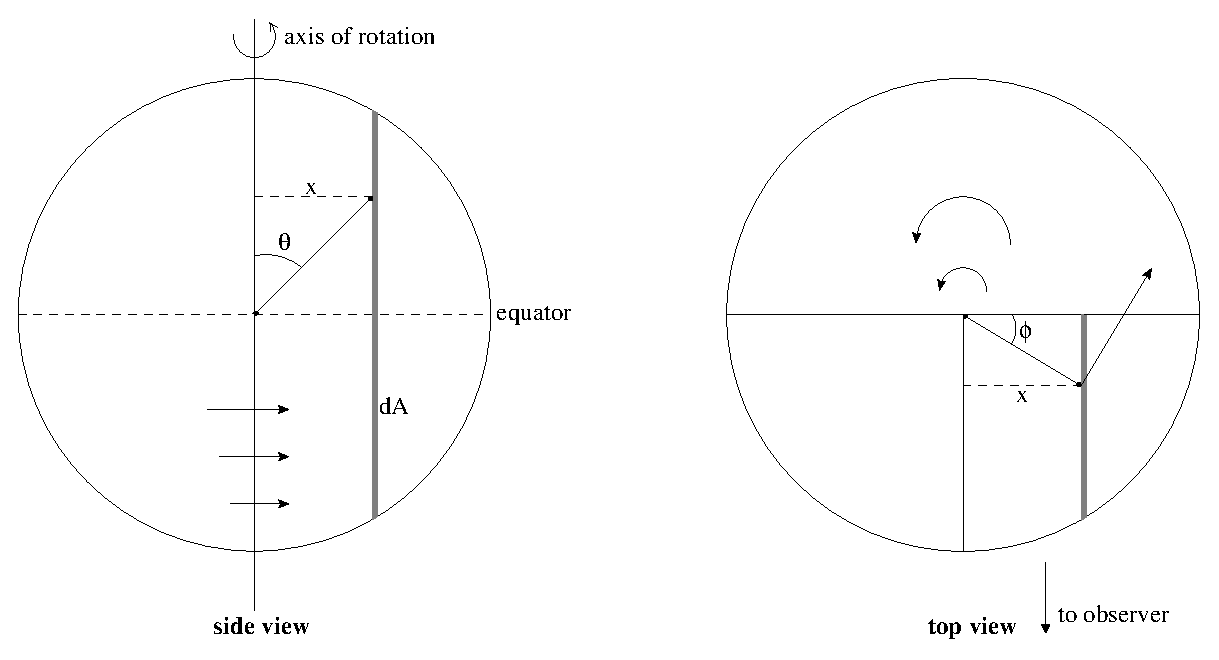
\includegraphics[width=12cm]{figs/rotational-broadening}
  \caption{Geometry for rotational broadening
  \label{fig:rot_broad}}
\end{figure*}
%%%%%%%%%%%%%%%%%%%%%%%%%%%%%%%%%%%%%%%%%%%%%%%%%%%%%%


If the resolution element of our telescope is so big we cannot resolve  the object of interest we need to take the systematic motion into account. This depends obviously on the type of object. As the most important example we will examine the observed broadening of spectral lines due to the rotation of stars. We assume that the star is spherical, and rotates rigidly which means any part of the star has the same angular speed $\omega$. The star is also assumed to be an isotropic radiator, and thus does not show limb darkening. We now need to derive the velocity distribution of all points on the star as seen from the observer. The geometry of the problem is shown in Figure~\ref{fig:rot_broad}.

The speed of a point on the stellar surface is given by
\be
v(\theta) = \omega R_\star \sin{\theta},
\ee
with $R_\star$ the radius of the star. The projection of this speed along the line of sight is given by
\be
v_{||} = \omega R_\star \sin{\theta} \cos{\phi}.
\ee
Because $R_\star \sin{\theta} \cos{\phi}$ is just the Cartesian $x$-coordinate of the point, this proves that all points on the stellar surface with the same $x$-coordinate have the same line-of-sight velocity 
\be
v_{||} = \omega x = v_\star \frac{x}{R_\star},
\ee
where $v_\star$ is the speed of the stellar surface at the equator. If the rotation axis of the star does not have a 90-degree angle with the line of sight, but a smaller angle $i$, we need to take into account another factor $\sin{i}$:
\be
v_{||} = v_\star \sin{i} \frac{x}{R_\star}.
\ee
Each stripe on the star has an area:
\be
\dd A = 2 \sqrt{R_\star^2- x^2} \, \dd x
\ee
so the fraction of the stellar disk with line of sight velocity $v_{||}$ is given by
\be
\dfrac{\dd A}{\int \dd A} = \dfrac{2 \sqrt{R_\star^2- x^2} \, \dd x}{\pi R_\star^2}.
\ee
Inserting
\be
x = \frac{R_\star}{v_\star \sin{i} } v_{||} 
\ee
yields the rotational profile:
\be
\phi(v_{||}) = \frac{2}{\pi v_\star \sin{i}} \sqrt{1 - \left( \frac{v_{||}}{v_\star \sin{i}} \right)^2 },
\ee
where $v_{||} \le v_\star \sin{i}$. To convert to frequency units we use the now familiar 
trick of using $(\nu-\nu_0) / \nu_0 = v_{||}/c$ to get:
\be
\phi(\nu) = \frac{2}{\pi \Delta \nu_\mathrm{max}} \sqrt{1 - \left( \frac{\nu-\nu_0}{\Delta \nu_\mathrm{max}} \right)^2 },
\ee
where
\be
\Delta \nu_\mathrm{max} = \nu_0 \frac{v_\star \sin{i} }{c}.
\ee

%%%%%%%%%%%%%%%%%%%%%%%%%%%%%%%%%%%%%%%%%%%%%%%%%%%%%%
   \begin{figure*}
   \centering
   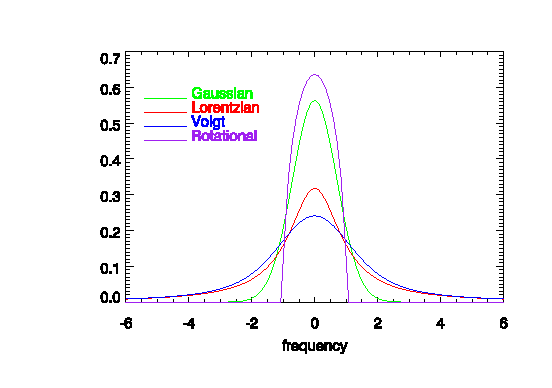
\includegraphics[width=12cm]{figs/profiles}
    \caption{Various broadening profiles. The frequency is given in different units for each profile in order to give them similar widths. The Gaussian and Voigt profiles are given as functions of frequency in Doppler width $\dnud$. The Lorentzian has $\gamma = 4 \pi$. The Voigt profile has $a=1$. The rotational profile has  $\Delta \nu_\mathrm{max} =1$.
    \label{fig:profiles}}
    \end{figure*}
%%%%%%%%%%%%%%%%%%%%%%%%%%%%%%%%%%%%%%%%%%%%%%%%%%%%%%

%%%%%%%%%%%%%%%%%%%%%%%%%%%%%%%%%%%%%%%%%%%%%%%%%%%%%%
\paragraph{Instrumental broadening}
For spectral lines that are narrow compared to the resolution of the spectrograph, the observed line profile is influenced by the instrument. Like other broadening mechanisms this broadening can be described by a line-spread function (LSF) that can look like anything, but is often well-approximated by a Gaussian function. The full-width-at-half-maximum (FWHM) of the LSF is called the spectral resolution. However, the spectral resolution is often specified as a quantity $R$:
\be
R = \frac{\lambda}{\mathrm{FWHM}} = \frac{c}{\Delta v},
\ee
since $R$ is often nearly constant with variations in $\lambda$. Low resolution spectrographs have $R\sim200$, while high resolution instruments have $R=10^4 - 10^5$. Optical spectrographs rarely have $R \geq 10^6$ and are then called ``ultra high resolution'' spectrographs, while in the radio regime spectrometers with $R>10^6$ are common.

%%%%%%%%%%%%%%%%%%%%%%%%%%%%%%%%%%%%%%%%%%%%%%%%%%%%%%
\subsection{Combining broadening mechanisms} \label{subsec:combining_broadening}

So far we have considered line profiles from different processes separately. Combining the various processes is simply done by convolving the profiles. If we have two broadening processes $\phi(\nu)$ and $\psi(\nu)$ are operating together then the resulting line profile is
\bea
\rho(\nu) &=& \phi(\nu) * \psi(\nu) =\psi(\nu) * \phi(\nu) \nonumber \\
&= &\int_{-\infty}^\infty \phi(\nu') \, \psi(\nu-\nu') \, \dd \nu' =
 \int_{-\infty}^\infty \phi(\nu-\nu') \,  \psi(\nu) \, \dd \nu'.
\eea

Convolutions can be performed multiple times after each other to include more than two processes. The convolution operation preserves the integral of the functions:
\be
\int_{-\infty}^\infty \phi(\nu) * \psi(\nu) \, \dd \nu = 
	\left( \int_{-\infty}^\infty \phi(\nu)  \, \dd \nu \right) \left( \int_{-\infty}^\infty \psi(\nu) \, \dd \nu \right).
\ee
This means that the convolution of two normalized line profiles is also normalized. This means as long as one is interested in line-integrated intensities only, it does not matter whether the spectrograph can resolve the line profile, the measured line-integrated intensity does not depend on the resolution of the instrument.

The convolution of two Lorentzians is a new Lorentzian with a FWHM $\gamma = \gamma_1 + \gamma_2$.
The convolution of two Gaussian functions is a new Gaussian with a width $\Delta \nu^2 = \Delta \nu_1^2 +  \Delta \nu_2^2$. Thus, when combining thermal and Doppler broadening the total profile function is given by a Gaussian with a width of
\be
\Delta \nu =  \frac{\nu_0}{c} \sqrt{\frac{2kT}{m} + \xi^2}.
\ee

The convolution of a Gaussian and a Lorentzian is called a Voigt function. There is no closed analytical form for this function. The corresponding profile function is
\be
\phi(\nu-\nu_0) = \frac{H(a,v)}{\sqrt{\pi} \dnud},
\ee
where
\bea
 H(a,v)&=&  \frac{a}{\pi} \int_{-\infty}^\infty \frac{\exp^{-y^2}}{(v-y)^2 + a^2 } \, \dd y\nonumber \\
 v&=& \frac{\nu-\nu_0}{\dnud}\nonumber \\
 a &=& \frac{\gamma}{4 \pi \dnud}
\eea
If $a \ll 1$ then the function looks like a Gaussian close to the central frequency, and like a Lorentzian in the line wings. The Voigt function is very important in modelling spectral lines in stellar atmospheres as it describes the combined action of natural broadening, collisional broadening, thermal broadening and possibly turbulence.

%%%%%%%%%%%%%%%%%%%%%%%%%%%%%%%%%%%%%%%%%%%%%%%%%%%%%%
\subsection{Line widths as a diagnostic}
%%%%%%%%%%%%%%%%%%%%%%%%%%%%%%%%%%%%%%%%%%%%%%%%%%%%%%

%%%%%%%%%%%%%%%%%%%%%%%%%%%%%%%%%%%%%%%%%%%%%%%%%%%%%%
   \begin{figure*}
   \centering
   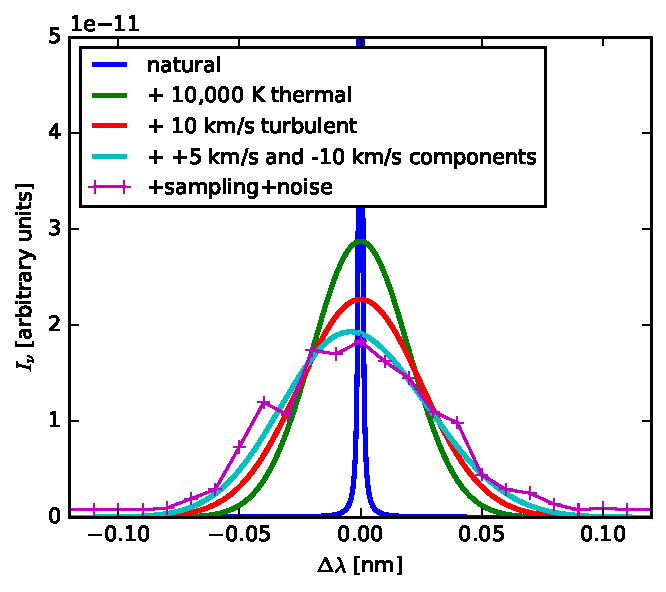
\includegraphics[width=10cm]{figs/line_broadening.pdf}
    \caption{Example intensities of the H$\alpha$ line as received from an optically thin source. Blue: the unrealistic case of natural broadening only. Because the profile is narrow its maximum value is $7\times10^{-9}$. Green: natural broadening and thermal broadening corresponding to  a temperature of 10,000~K. Red: As the green curve but now also including 10~km~s$^{-1}$ microturbulence. Cyan: resulting line profile of two clouds with individual line profiles as the red curve, one cloud moving at a line-of-sight velocity of +5 and one of -10~km~s$^{-1}$. Purple: as the cyan curve, but now taking into account finite spectrograph resolution and photon noise where the maximum intensity has an expectation value of 100 photons.}
    \label{fig:line_broadening}
    \end{figure*}
%%%%%%%%%%%%%%%%%%%%%%%%%%%%%%%%%%%%%%%%%%%%%%%%%%%%%%

Line broadening typically depends on multiple quantities. Using the line width of a single line as a diagnostic of the source is therefore often difficult or even impossible. Not all lines are equally sensitive to the parameters that set the line broadening, so one can exploit observations of multiple lines from the same source to disentangle the various contributions to the line broadening. A very useful example is to use observations of two spectral lines from two atoms with different mass to disentangle thermal and turbulent broadening. The thermal broadening depends on the mass of the atom, while the turbulent broadening only depends on the bulk velocities, and so is the same for all atomic species.

Assume we observe two spectral lines from a source that is optically thin at all relevant wavelengths, so that the shape of the spectral lines is proportional to the line profile function: $\Inu \sim \phi_\nu$. Assume that the dominant two sources of broadening are thermal broadening and turbulent broadening. The thermal width in velocity units is $\sqrt{2kT/m_i}$ with $i=1,2$ denoting the atomic species, while the turbulent width in velocity units is just $\xi$. Denote the observed width of spectral line 1 caused by atom 1 as $\Delta w_1$, and likewise for line two. Then
\bea
\Delta w^2_1 &=& \frac{2kT}{m_1} + \xi^2, \label{eq:twoline1} \\
\Delta w^2_2 &=& \frac{2kT}{m_2} + \xi^2, \label{eq:twoline2}
\eea
Let $m_2 = x m_1$, so that
\bea
\Delta w^2_1 - \Delta w^2_2 &=&  \frac{2kT}{m_1} \left( 1 - \frac{1}{x} \right) \\
 T &=& \left( \Delta w^2_1 - \Delta w^2_2 \right) \frac{m_1}{2 k} \frac{x}{x-1}.
\eea
The turbulent velocity $\xi$ can then be directly computed from Eqs.~\ref{eq:twoline1} or~\ref{eq:twoline2}.


%%%%%%%%%%%%%%%%%%%%%%%%%%%%%%%%%%%%%%%%%%%%%%%%%%%%%%
\section{Bound-free transitions}

If a collision or photon causes a transition from a bound to an unbound state, we call this a bound-free transition. The canonical example is ionisation of an atom, where part of the absorbed energy is used to release an electron from the potential well of the rest of the atom, and the leftover energy is put into kinetic energy. As for bound-bound transitions, there are five processes:

\begin{itemize}
\item radiative ionization
\item spontaneous radiative recombination
\item induced radiative recombination
\item collisional ionization
\item collisional recombination
\end{itemize}

It is possible to go through the same process as for bound-bound transitions and derive the expressions for extinction, emissivity and the rate coefficients, as well as the Einstein-Milne relations, which are the bound-free equivalent of the Einstein relations. We will however just give the results here and argue heuristically why the expressions are plausible.

%%%%%%%%%%%%%%%%%%%%%%%%%%%%%%%%%%%%%%%%%%%%%%%%%%%%%%
\paragraph{Collisional ionisation and recombination}

We start with collisional processes. Collisional ionisation requires a colliding particle (often an electron) of sufficient energy. The formalism is entirely analogous to bound-bound collisions, so if the velocity distribution is Maxwellian, it has an ionisation rate per particle in state $i$ to the ground state of the next ion $c$ per second of
\be
C_{ic} = n_\mathrm{e} f_\mathrm{ioniz}(T),
\ee
where $f_\mathrm{ioniz}(T)$ depends on the atom and transition under consideration.

Collisional recombination is a three-body process, it requires an ion, an electron that gets captured and a third particle (often an electron) to carry away the excess energy and fulfil momentum conservation. The rate per particle per second is
\be
C_{ci} = n^2_\mathrm{e} f_\mathrm{recom}(T).
\ee
Because it requires three particles to be close to each other at the same time this process is often not very important. The rate coefficients are related because they must yield the Saha distribution for particles in thermal equilibrium:
\be
\left. \frac{n_c}{n_i} \right|_\mathrm{LTE}   =  \frac{C_{ic}}{C_{ci}}
\ee 

%%%%%%%%%%%%%%%%%%%%%%%%%%%%%%%%%%%%%%%%%%%%%%%%%%%%%%
\paragraph{Radiative ionisation}

Radiative ionisation is also called photoionisation. If a particle is hit by a photon of sufficient energy it can be ionised. The cross section for this process per particle in a given state at a given frequency is $\sigma_{ic}(\nu)$. The rate per second per particle in state $i$ is thus
\be
R_{ic} = \int_{\nu_0}^\infty \frac{4 \pi}{h \nu} \sigma_{ic}(\nu) \Jnu \, \dd \nu,
\ee
where $\nu_0$ is the frequency corresponding to the energy difference between state $i$ and the continuum. The ionisation cross section is often largest close to $\nu_0$ and gets smaller for higher frequencies.

%%%%%%%%%%%%%%%%%%%%%%%%%%%%%%%%%%%%%%%%%%%%%%%%%%%%%%
\paragraph{Radiative recombination}

Spontaneous radiative recombination requires the presence of an ion and an electron. The rate per particle per second is given by
\be
R^\mathrm{spont}_{ci} = \nelec \int_{0}^\infty v \, f(v) \sigma_{ci}^\mathrm{spont}(v) \, \dd v,
\ee
where $f(v)$ is the velocity distribution of the electrons. If the Maxwell distribution holds then the integral can in principle be performed to yield a simple relation for the rate per particle:
\be
R^\mathrm{spont}_{ci} = N_\mathrm{e} \, \alpha_i(T).
\ee
Here $\alpha_i(T)$ is a recombination coefficient with units [m$^3$ s$^{-1}$], and depends on the temperature of the gas.

Without proof we give the total radiative recombination rate per particle in state $c$ per second, combining both spontaneous and induced recombination, and expressed using only the cross section of radiative ionisation:
\be \label{eq:recrate}
R_{ci} = 4 \pi \left[ \frac{n_i}{n_c}\right]_\mathrm{LTE} \int_{\nu_0}^\infty \frac{\sigma_{ic}(\nu)}{h \nu}
\left( \frac{2 h \nu^3}{c^2}+ \Jnu \right) \exp^{-h\nu/kT} \, \dd \nu.
\ee
The term $\left[ n_i/n_c\right]_\mathrm{LTE}$ can be computed from the Saha relation and appears because of the Einstein-Milne relations, the equivalent of the Einstein relations but for bound-free transitions. The $2 h \nu^3/c^2$ term is for spontaneous recombination, while the $\Jnu$ term represents induced recombination. Note that $R_{ci}$ still depends on the electron density, but the explicit dependency is hidden in $\left[ n_i/n_c\right]_\mathrm{LTE}$.

The bound-free extinction coefficient  and source function are 
\bea
\anu^{\mathrm{bf}} &=& n_i \sigma_{ic}(\nu) (1-\frac{b_c}{b_i} \exp^{- h\nu/kT}) \nonumber, \\
\Snu^{\mathrm{bf}} &=& \frac{2h \nu^3}{c^2} \dfrac{1}{\dfrac{b_i}{b_c} \exp^{h\nu/kT}-1}.
\eea
The $b_i$ and $b_c$ symbols are called departure coefficients, and are defined as the ratio of the actual level population to the LTE level population:
\be
b_i = \frac{n_i}{n_i^\mathrm{LTE}}
\ee

%%%%%%%%%%%%%%%%%%%%%%%%%%%%%%%%%%%%%%%%%%%%%%%%%%%%%%
\subsection{Ionisation equilibrium around a hot star}

As an example we treat the ionisation equilibrium of the interstellar medium (ISM) around a hot star. The ISM is assumed to be tenuous, so that collisional processes are negligible, and consists of hydrogen only. We also assume induced recombination is negligible. The ionisation equilibrium can then be described by a rate equation balancing the rate of photo-ionisation to the rate of spontaneous recombination. We furthermore assume that the excited states of neutral hydrogen have negligible populations. This means that all photoionisation happens from the ground state, the rate equation is thus:
\bea
\nHI\, R_\mathrm{ion}  &=&  \nHII \, R_\mathrm{rec} \\
\nHI\,  \int_{\nu_0}^\infty \frac{4 \pi}{h \nu} \sigma_{1c}(\nu) \Jnu \, \dd \nu & = &
\nHII\, n_\mathrm{e} \, \sum_i \alpha_i(T).
\eea
This equation must be supplemented by the particle conservation equation:
\be
\nHI + \nHII = n_\mathrm{H}.
\ee

The sum is over all energy levels in neutral hydrogen, and often just written $\alpha(T) =\sum_i \alpha_i(T)$. But there is a special case here. A recombination to the ground level $i=1$ emits a photon with sufficient energy to ionise another atom. If this ionisation occurs close-by, the recombination to the ground level and the subsequent ionisation cancel each other out. This is called the ``on the spot'' approximation. Instead of $\alpha(T)$ we should use an effective recombination rate 
\be
\sum_{i>1} \alpha_i(T) = \alpha(T)-\alpha_1(T)  = \beta(T)
\ee

In addition we assume that all radiation is coming from the star, and at large distance we have
\be
4 \pi \Jnu = \frac{L_\nu}{4 \pi r^2}.
\ee


%%%%%%%%%%%%%%%%%%%%%%%%%%%%%%%%%%%
    \begin{figure*}
    \centering
   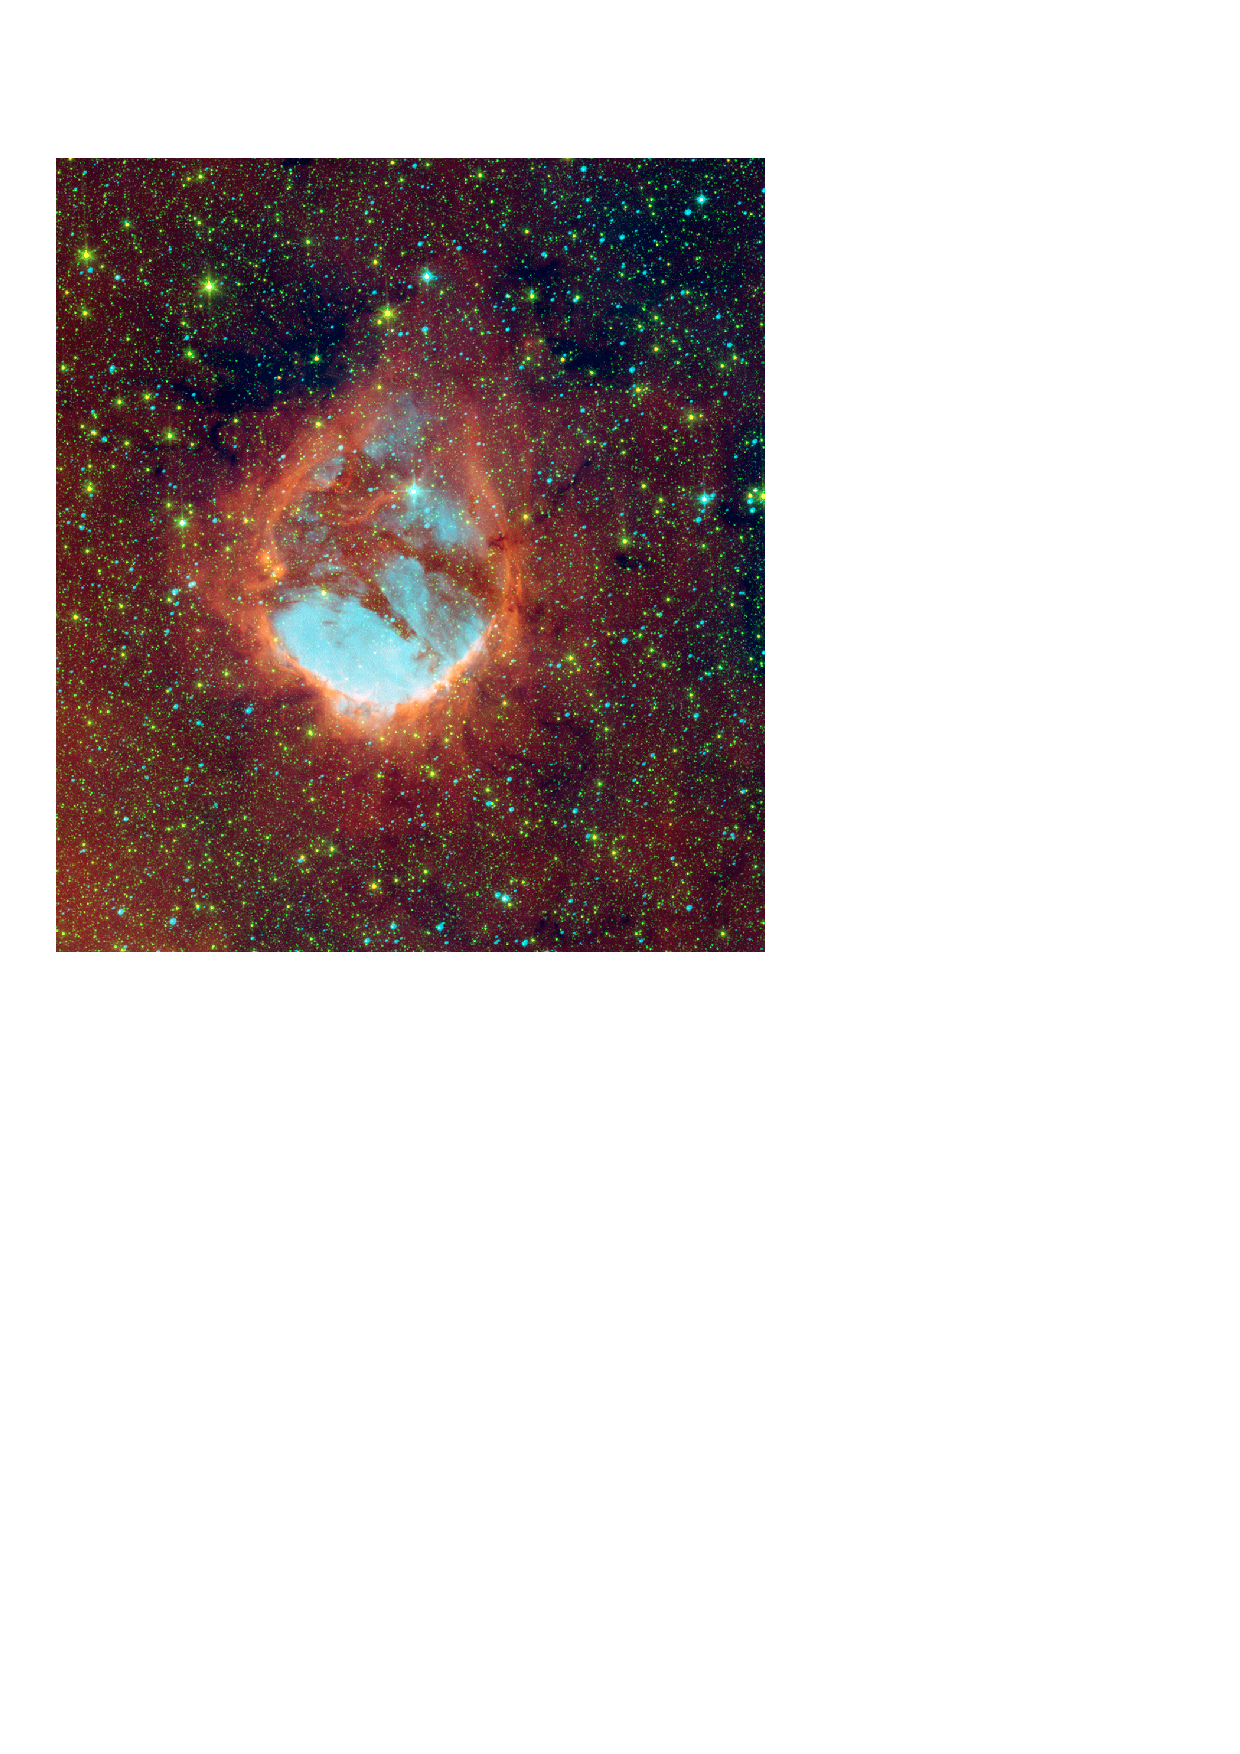
\includegraphics[width=12cm]{figs/RCW120}
    \caption{False color image of the \HII\ region RCW120. The turquiose color shows H$\alpha$ radiation caused by recombination cascades inside the ionized bubble. The orange color displays 8 $\mu$m emission, which is dominated by polycyclic aromatic hydrocarbon molecules. The \HII\ region is ionized by an O8 V star and is approximately 6 light year in diameter. Image taken from~\citet{2007A&A...472..835Z}.}
     \label{fig:RCW120}
    \end{figure*}
 %%%%%%%%%%%%%%%%%%%%%%%%%%%%%%%%%%%%

\paragraph{Example} Let us  now make a rough estimate of the ionisation condition in a hydrogen nebula around a hot star. We use the following approximate values:
\begin{itemize}
\item $n_\mathrm{H} = 10^7$~m$^{-3}$,
\item The number of ionising photons from the star is $S_\star = \int_{\nu_0}^\infty \frac{L_\nu}{h \nu} \, \dd \nu = 5 \times 10^{48}  $ photons s$^{-1}$. This corresponds to an O6V star, i.e., a hot giant.
\item the typical photoionisation cross section is $\sigma = 6 \times 10^{-22}$ m$^{2}$,
\item typical recombination cross section $\beta(T) = 4  \times 10^{-19}$ m$^{3}$ s$^{-1}$.
\end{itemize}

We now ask ourself the question: what is the neutral fraction $\xi= \nHI/(\nHI + \nHII)$ at a distance of $r=5$~parsecs from the star. The flux of ionising photons at this distance is
\be
\frac{S_\star}{4 \pi r^2} = 2 \times 10^{13}\ \mathrm{m}^{-2} \ \mathrm{s}^{-1}.
\ee
The ionisation rate per neutral hydrogen atom is given by
\be
\int_{\nu_0}^\infty \frac{4 \pi \Jnu }{h \nu} \sigma_{ic}(\nu) \, \dd \nu \approx \frac{S_\star}{4 \pi r^2} \sigma = 10^{-8} \ \mathrm{s}^{-1} = R_\mathrm{ion}.
\ee
Note that this implies that a freshly recombined neutral atom will remain on average neutral for a time $t=1/R_\mathrm{ion}\approx 3.2$~year before it is ionised again.

We assume the gas is composed of hydrogen only, thus $N_\mathrm{e} = n_\mathrm{H\, II}$, and the rate equation becomes:
\be \label{eq:HII_ion_rate}
\nHI R_\mathrm{ion} = n_\mathrm{H\, II}^2 \beta.
\ee
We now define the hydrogen neutral fraction $\xi$ as
\be
\xi = \frac{\nHI}{\nH}
\ee
and we can write 
\bea
\nHI &=& \xi \nH, \nonumber \\
\nHII &=& (1-\xi) \nH.
\eea
We plug this into Eq.~\ref{eq:HII_ion_rate} to get
\be
R_\mathrm{ion} \nH \xi =  \beta \nH^2 (1-\xi)^2.
\ee
Solving for $\xi$ yields
\be
\xi = \frac{\nH \beta}{R_\mathrm{ion}} = 4 \times 10^{-4}.
\ee
So the gas is almost completely ionised at 5 parsec from the central star. We can now also estimate how long the gas will remain ionised if the central star would suddenly be switched off: $t=1/(\nelec \beta) \approx 10^4$~year.

At distances smaller than 5 parsec the ISM is even more ionised because of the higher photon flux. But at some distance from the star the ISM must turn neutral. We can estimate the distance over which the ISM goes from ionised ($\xi \ll 1$) to neutral ($\xi \approx 1$) by computing the mean free path of an ionising photon when $\xi=0.5$. The mean free path is
\be
l = \frac{1}{\anu} \approx \frac{1}{\xi \nH \sigma} \approx 0.01~\mathrm{parsec}.
\ee 
This change is very abrupt compared to the fact that up to at least 5~parsec the ISM is ionised. What happens is that once the flux from the star is so low that it cannot maintain full ionisation, the mean free path drops, so the ionising photons get absorbed quicker, leading to a larger neutral fraction and even more absorption. This process is sometimes called self shielding.

The abrupt change allows us to consider a simple picture where the ISM around a hot star is fully ionised up to a radius $R_\mathrm{S}$ and neutral further away. The bubble of ionised material is called a Str\"omgren sphere. The number of recombinations per second in the sphere is 
\be
\frac{4 \pi R_\mathrm{S}^3}{3} \nH^2 \beta.
\ee
But because  each recombination must be balanced by a photo-ionisation this must be equal to the total number of ionising photons emitted per second by the star $S_\star$. Equation the two and solving for $R_\mathrm{S}$ yields:
\be
R_\mathrm{S} = \left( \frac{3}{4\pi} \frac{S_\star}{\nH^2 \beta} \right)^{1/3}.
\ee
This radius is called the Str\"omgren radius. For our example case it is about 10~parsec. Note that the volume of the Str\"omgren sphere $V \sim R_\mathrm{S}^3 \sim \nH^{-2}$. If the ISM is twice as dense the volume decreases by a factor 4 and not a factor 2 as you might think. The reason is that the recombination rate is quadratic in the particle density (you need one electron and one proton to recombine), so twice the density requires 4 times as many ionising photons to keep the gas ionised.

\section{Other radiative processes}
In most circumstances we are interested in the bound-bound and bound-free transitions. There exist however many more processes that can lead to photon absorption and emission. We briefly treat a few of the more common ones.

\paragraph{Free-free transitions}

%%%%%%%%%%%%%%%%%%%%%%%%%%%%%%%%%%%
    \begin{figure*}
    \centering
   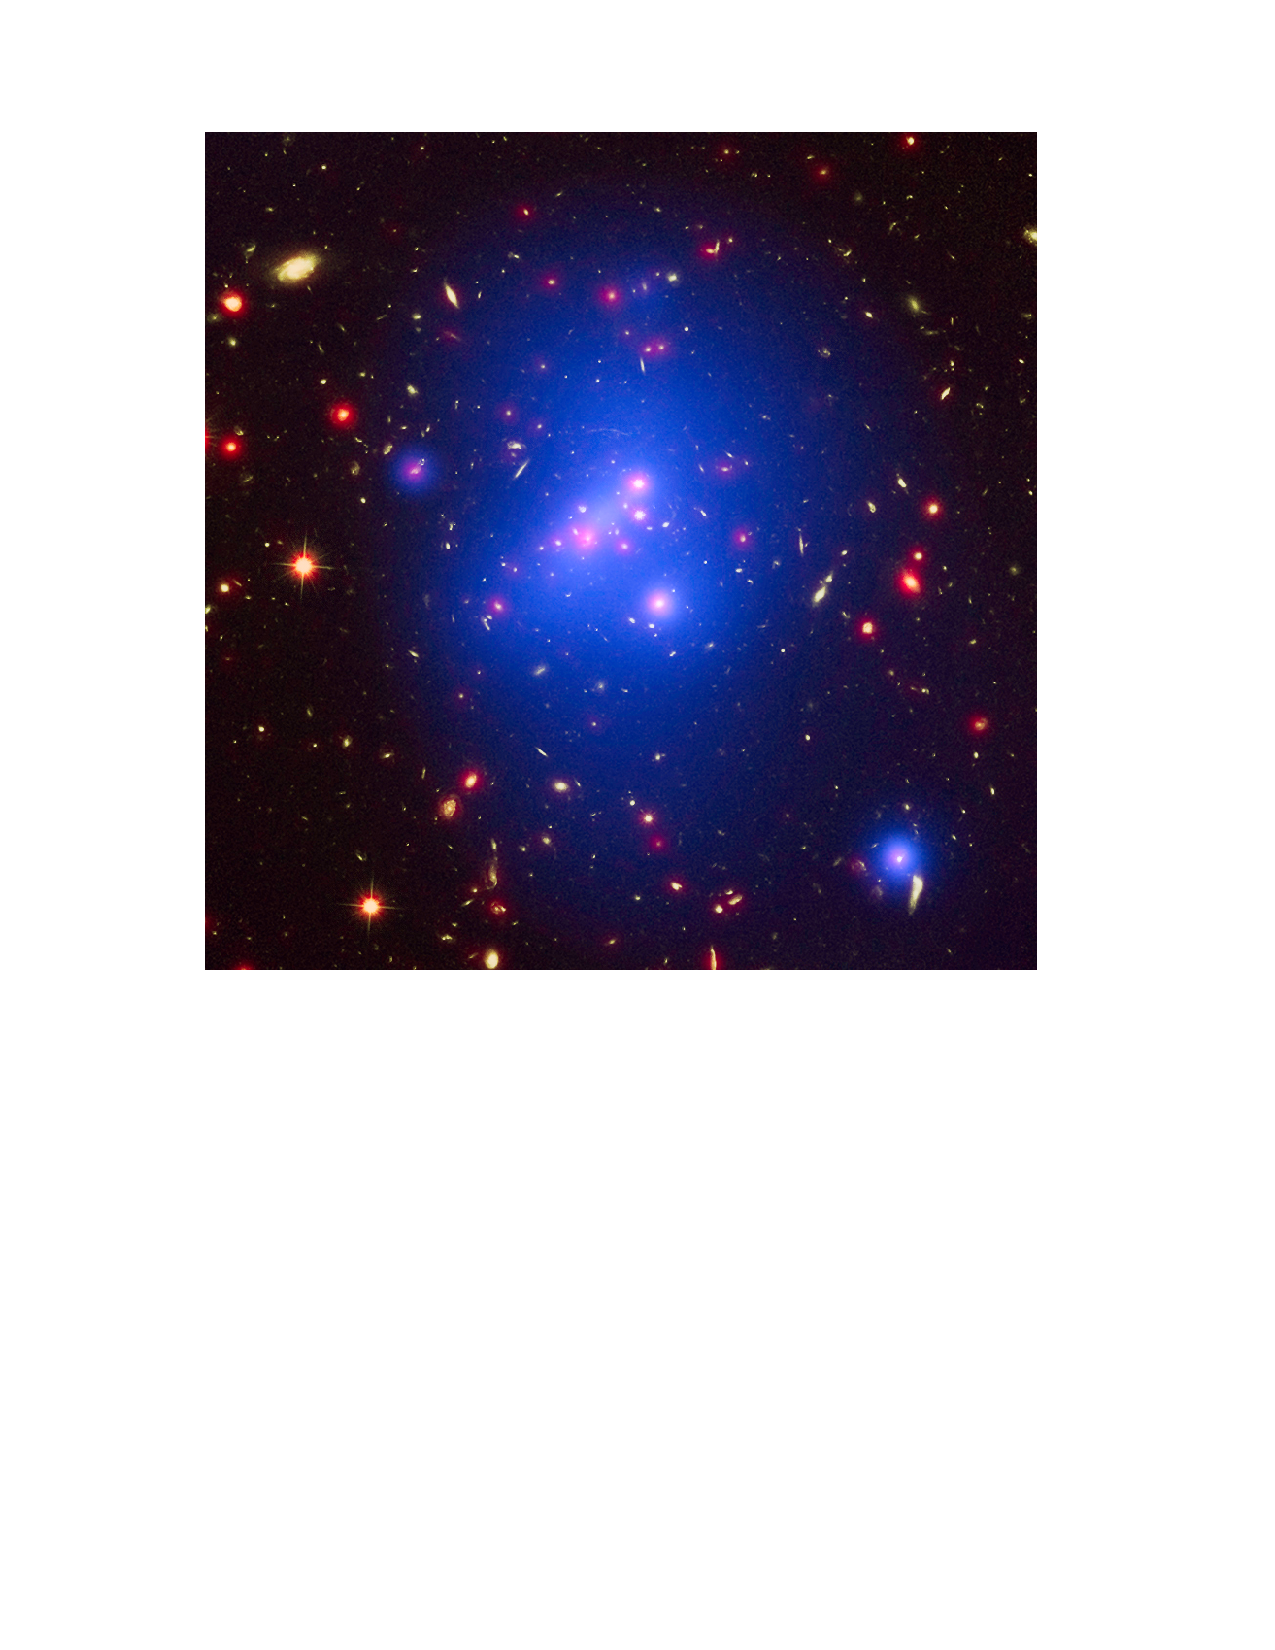
\includegraphics[width=12cm]{figs/galaxy_cluster}
    \caption{IDCS J1426.5+3508: A massive galaxy cluster located about $10^{10}$ light years from Earth. The stars in the galaxies are visible in the the optical Hubble and infrared Spitzer images (yellow and red). The diffuse blue glow is X-ray emission observed with Chandra. From fits to the spectrum of the X-ray radiation the temperature of the gas is estimated to be $\sim 7\times 10^7$~K.
    Image taken from \url{http://chandra.harvard.edu}, scientific results using the data are presented in \citet{2016ApJ...817..122B}.}
     \label{fig:galaxy_cluster}
    \end{figure*}
 %%%%%%%%%%%%%%%%%%%%%%%%%%%%%%%%%%%%
 
A free-free transition is the emission or absorption of a photon by an electron that moves in the electric field of a charged particle. If the particle velocities follow the Maxwell distribution then the emissivity is given by
\be
j^\mathrm{ff}_\nu = \frac{8e^6}{3 m c^3} \left( \frac{2 \pi}{3 k \me}\right)^{1/2} \nelec n_\mathrm{ion} \frac{Z^2}{\sqrt{T} } \exp^{-h \nu /kT} \bar{g}_\mathrm{ff},
\ee
with $Z$ the charge of the particle in elementary charges and $\bar{g}_\mathrm{ff}$ a so-called {\it velocity averaged Gaunt factor} which depends on frequency and temperature. The source function is the Planck function, and we can thus compute the corresponding extinction coefficient from $\anu= \jnu/\Bnu$:
\be
\alpha^\mathrm{ff}_\nu = \frac{4e^6}{3mhc} \left( \frac{2 \pi}{3 k \me}\right)^{1/2}  \nelec n_\mathrm{ion} \frac{Z^2}{\sqrt{T} \nu^3} (1-\exp^{-h \nu /kT}) \bar{g}_\mathrm{ff},
\ee
with $Z$ the ion charge and $g_\mathrm{ff}$ a quantum mechanical correction factor. The source function is the Planck function as long as the Maxwell distribution holds. Emission from this process is also called `thermal bremsstrahlung'. For optically thin emission the spectrum is proportional to $j^\mathrm{ff}_\nu$. The location of the cutoff caused by the $\exp^{-h \nu /kT}$ term is a temperature diagnostic of the emitting gas.

\subsection{Elastic scattering}

Elastic scattering processes are processes where a photon is scattered, meaning that it changes its direction, but does not change its frequency.

\paragraph{Thomson scattering} Scattering of photons by free electrons is called Thomson scattering. Its extinction coefficient is independent of frequency and is given by
\be
\anu = \sigma^\mathrm{T} \nelec = 6.65 \times 10^{-29}\ \mathrm{m}^{-2} \  \nelec.
\ee
Its source function is, assuming isotropic scattering: $\Snu^\mathrm{T} = \Jnu$, which is frequency-dependent.

This expression is valid for low-energy photons and electrons.  At relativistic speeds the correct description is Compton scattering. Thomson scattering is the dominant source of continuum opacity in hot stars, where hydrogen is almost completely ionised. It also causes the solar corona to scatter the light from the solar photosphere and gives rise to the so-called {\it white-light corona}.

\paragraph{Rayleigh scattering}
Photons can also scatter on electrons bound in an atom or molecule. If $\nu \ll \nu_0$ then the cross section per particle is given by
\be
 \sigma^\mathrm{R}_\nu = f_{lu} \sigma^\mathrm{T}  \left( \frac{\nu}{\nu_0} \right)^4,
\ee
with $f_{lu}$ and $\nu_0$ the oscillator strength and frequency of the transition. Again $\Snu=\Jnu$. Rayleigh scattering is often unimportant in stars, but it causes the blue color of the sky on Earth.

\subsection{The H$^-$ ion}
If one adds the various sources of bound-free and free-free extinction coefficients together for the atmosphere of cool stars like the Sun, then one finds that it is much lower than what is expected. It  turns out that a rather unusual particle is responsible for most of the continuum opacity here, the negative ion of hydrogen H$^-$, which is a neutral hydrogen atom with an extra electron. It has only one bound state, with a binding energy of $E_\infty-E_1 =0.75$~eV, corresponding to a wavelength of $\lambda=1650$~nm. There is only one bound state, so H$^-$ has no spectral lines. 

The bound-free transition coefficient is the dominant source of continuum opacity between the Balmer edge at 365~nm and 1600~nm. At longer wavelengths H$^-$ free-free radiation is the dominant continuum process.  Note that H$^-$ free-free means a neutral hydrogen interacting with a free electron. 

Hydrogen is almost completely neutral in the photosphere of cool stars, so where do the electrons come from that are needed to make H$^-$? It turns out that other elements such as Na, Mg, Si, and Fe have a low first ionisation potential and are still singly ionised in the photosphere of such cool stars. Even though their abundance is low (roughly one particle per one million hydrogen atoms) they still provide the sufficient electrons to make H$^-$ the dominant source of opacity.

%%%%%%%%%%%%%%%%%%%%%%%%%%%%%%%%%%%%%%%%%%%%%%%%%%%%%%
\section{Rate equations}

\subsection{General theory}

In the previous sections we have found expressions for rate coefficients: expressions that give the probability per particle in state $i$ per second to transition to state $j$. If the rates between the states of a particle are known we can set up an equation system that determines the population of the states. For each state we have:
\be
\frac{\dd n_i}{\dd t} = \mathrm{rates\ into\ level\ } i - \mathrm{rates\ out\ of\ level\ }i
\ee

We furthermore assume that the system is in equilibrium, so that the time derivative is zero. The rates in and out of the level balance in that case. Denote the rate coefficient from $i$ to $j$ as $P_{ij}$ (with units s$^{-1}$) and we consider a particle with $N$ states in total. Then the rate equation for level $i$ is 
\be
\sum_{j, j \neq i} n_j P_{ji} - n_i \sum_{j, j \neq i} P_{ij} = 0.
\ee
This equation can be written in an elegant matrix form. Define
\be
P_{ii} = - \sum_{j, j \neq i} P_{ij},
\ee
which means the total rate coefficient out of level $i$. Then the rate equations are 
\be
P \vec{n}= 0,
\ee
where $P$ is a matrix whose elements are $P_{ij}$ and $\vec{n}$ is a vector whose components $n_i$ are the populations of each level $i$. There are only $N-1$ independent equations, so we should replace one equation with particle conservation:
\be
\sum_{i=1,N} n_i = n_\mathrm{tot}.
\ee
In the matrix form of the equations this means we set $P_{ij} =1$ in one row of the rate matrix, and replace the zero with $n_\mathrm{tot}$ in the corresponding element on right hand side. 

\subsection{The two-level atom}
In order to make this less abstract we look at a two-level atom with a bound-bound transition between the levels and $E_2>E_1$. 

The rate equation for level 1 is :
\be
 n_2 P_{21} - n_1 P_{12} = 0.
\ee
The rate equation for level 2 is :
\be
 n_1 P_{12} - n_2 P_{21} = 0.
\ee
We need to replace one of the equations with particle conservation:
\be
n_1 + n_2 = n_\mathrm{tot}.
\ee
We can thus write the rate equations in matrix form as
\be
\begin{bmatrix}
  P_{12} & P_{21} \\
  1 & 1
 \end{bmatrix}
 \begin{bmatrix}
  n_1 \\
  n_2
 \end{bmatrix}
 =
  \begin{bmatrix}
  0 \\
  n_\mathrm{tot}
 \end{bmatrix}
\ee
This system has the solution
\be
\begin{bmatrix}
  n_1 \\
  n_2
 \end{bmatrix}
 =
  \begin{bmatrix}
   (n_\mathrm{tot} P_{21})/(P_{12}+P_{21}) \\
  (n_\mathrm{tot} P_{12})/(P_{12}+P_{21})
 \end{bmatrix}.
\ee
A more illuminating form is :
\be
\frac{n_2}{n_1} = \frac{P_{12}}{P_{21}}.
\ee

We can now fill in explicit expressions for the rate coefficients using the five bound-bound processes:
\be
\frac{n_2}{n_1} = \frac{B_{12} \Jbar + C_{12}}{A_{21}+ B_{21} \Jbar + C_{21}}.
\ee
In the limit where collisions dominate the rate coefficients we get $n_2/n_1=C_{12}/C_{21}$, which, using the Einstein relations for collisions just reduces to the Boltzmann population ratio.
In the low density limit we ignore collisions to get
\bea
\frac{n_2}{n_1} &=& \frac{B_{12} \Jbar}{A_{21}+ B_{21} \Jbar}. \nonumber \\
                        &=& \frac{\Jbar}{A_{21}/B_{12} + (B_{21}/B_{12}) \Jbar} \nonumber \\
                        &=&\frac{g_2}{g_1} \frac{\Jbar}{ 2h\nu^3/c^2 + \Jbar}.	
\eea
In the last expression we filled in the Einstein relations, and $g_1$ and $G_2$ are the statistical weights of the levels. A further slight rearrangement gives
\be
\frac{g_1 n_2}{g_2 n_1} =  \frac{\Jbar}{ 2h\nu^3/c^2 + \Jbar} < 1.
\ee
From the discussion about  bound-bound transitions you remember that in order to get a negative extinction coefficient and thus laser action you need $(g_1 n_2)/(g_2 n_1) > 1$. 

This thus proves that it is impossible to create a laser, or have an astrophysical laser mechanism with a two-level system only: neither collisions nor a radiation field can set up the required population inversion.

\subsection{A three-level atom as a density diagnostic} 

In many astrophysical circumstances the radiation field $\Jbar$ is so weak that the terms involving the radiation field can be ignored in the rate equation. Let's take a look at a three level atom, with ground state $1$ and two excited levels 2 and 3. We assume both excited levels are only connected to the ground state, there are no transitions between the excited levels.
For level 2 we assume that $A_{21}$ is of the same order as $C_{21}$, but for level 3 we assume that  $A_{31} \gg C_{31}$.  Such a situation can arise if the transition from 2 to 1 is forbidden and the transition from 3 to 1 is allowed.
The rate equation for level 2 is now:
\bea
n_2 (C_{21}+A_{21}) &=& n_1 C_{12} \nonumber \\
n_2 &=& n_1 \frac{C_{12}}{C_{21}+A_{21}}.
\eea
And for level 3 it is simply:
\be
n_3=n_1 \frac{C_{13}}{A_{31}}.
\ee

We can now express the frequency-integrated emissivity of transition \mbox{$2 \rightarrow 1$ }as
\be
j_{21} = \frac{h \nu_{21}}{4 \pi} A_{21} n_2 =  \frac{h \nu_{21}}{4 \pi} n_1 A_{21} \frac{C_{12}}{C_{21}+A_{21}}.
\ee
We do the same for the other transition and compute the ratio of the emissivities:
\bea
\frac{j_{31}}{j_{21}} &=& \frac{\nu_{31}}{\nu_{21}} \frac{A_{31}}{A_{21}} \frac{C_{21}+A_{21}}{C_{12}} \frac{C_{13}}{A_{31}} \nonumber \\
&=& \frac{\nu_{31}}{\nu_{21}} \frac{C_{13}}{C_{12}} \left(1+\frac{C_{21}}{A_{21}} \right)
\eea
Remember that the collisional rate coefficient depends on the electron density as $C_{ij} = \nelec f_{ij}(T)$, where $f_{ij}(T)$ is a temperature-dependent function. We insert this expression into the equation for the emissivity ratio to make the electron dependence explicit:
\be \label{eq:linerat}
\frac{j_{31}}{j_{21}} = \frac{\nu_{31}}{\nu_{21}} \frac{f_{13}(T)}{f_{12}(T)} \left(1+\nelec\frac{f_{21}(T)}{A_{21}} \right).
\ee
 At low electron densities ($\nelec f_{21}(T) \ll A_{21}$) the ratio is not sensitive to the electron density. At very high electron densities the assumption that $A_{31} \gg C_{31}= \nelec f_{31}(T)$ breaks down, and we need to modify our model. But for intermediate electron densities where $\nelec \approx A_{21}/ f_{21}(T)$ our model works well. If we furthermore assume that the spectral lines form under optically thin conditions, then the observed flux ratio is equal to the emissivity ratio and we can directly apply Equation~\ref{eq:linerat} to estimate the electron density in the observed object.
 
In reality three-level atoms do not exist. Real atomic systems are much more complicated. But also in real atoms the basic concept described here can be used to estimate densities. The rate equations to solve become however more complicated and are typically solved numerically. 
 
  %%%%%%%%%%%%%%%%%%%%%%%%%%%%%%%%%%%%%%%%%%%%%%%%%%%%%%
 \subsection{A three-level atom as a temperature diagnostic}
   %%%%%%%%%%%%%%%%%%%%%%%%%%%%%%%%%%%%%%%%%%%%%%%%%%%%%%
   
  %%%%%%%%%%%%%%%%%%%%%%%%%%%%%%%%%%%%%%%%%%%%%%%%%%%%%%
\begin{figure*}
  \centering
  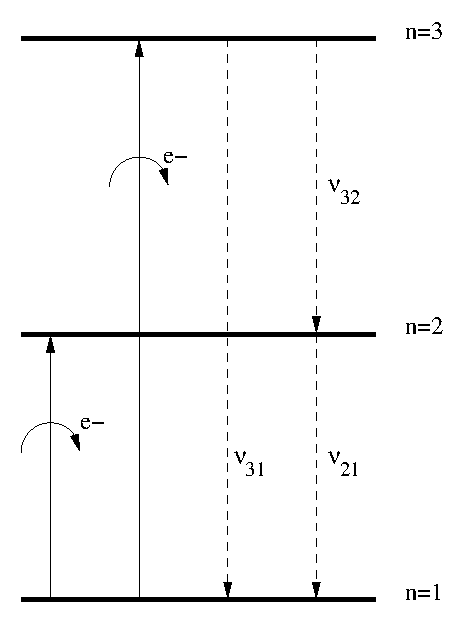
\includegraphics[width=6cm]{figs/three-level-atom}
  \caption{Schematic term diagram of the three-level atom as a temperature diagnostic. Horizontal lines indicate the energy of the states with $n=1$, $2$, and $3$, vertical solid lines indicate collisional excitation, vertical dashed lines spontaneous radiative deexcitation.}
  \label{fig:three-level-atom}
\end{figure*}
%%%%%%%%%%%%%%%%%%%%%%%%%%%%%%%%%%%%%%%%%%%%%%%%%%%%%%

 A three-level atom (or a suitable set of  three levels in a more complicated atom) can also be used as a temperature diagnostic. We consider the situation depicted in Figure~\ref{fig:three-level-atom}: the two excited levels 2 and 3 are only populated by collisional excitation from the ground state, and depopulated only by spontaneous deexcitation. This means we only consider low-density plasmas where $C_{ji} \ll A_{ji}$, with $j$ the upper and $i$ the lower level of the transition.

Again, we consider the rate equations for the excited levels. Level 3 is populated by collisions from the ground state and depopulated by radiative deexcitation to levels 1 and 2, so that:
\be
C_{13} n_1 = \left( A_{32} + A_{31} \right) n_3. \label{eq:tl-one}
\ee
Level 2 is populated by collisions from level 1 and radiative deexcitation from level 3, yielding:
\be
C_{12} n_1 + n_3 A_{32} = A_{21} n_2. \label{eq:tl-two}
\ee
The ratio of the frequency-integrated emissivities of the $3\rightarrow 2$ and $2\rightarrow 1$ transitions is 
\be
\frac{j_{21}}{j_{32}} = \frac{\nu_{21}}{\nu_{32}} \frac{A_{21} n_2}{A_{32} n_3}.
\ee
We then eliminate $A_{21} n_2$ using Eq.~\ref{eq:tl-two} and the ratio $n_1/n_3$ using Eq.~\ref{eq:tl-one} to arrive at
\be
\frac{j_{21}}{j_{31}} = \frac{\nu_{21}}{\nu_{32}} \left( 1 + \frac{C_{12}}{C_{13}} \frac{A_{31} + A_{32}}{A_{32}} \right). \label{eq:temp_diagnostic}
\ee
Collsional excitation coefficients can be written as
\be
C_{ij} = \nelec \, \Omega_{ij}(T) \, \sqrt{T} \, \exp^{ (E_i-E_j)/kT},
\ee
where $\Omega$ is a slowly varying function of temperature. If one can estimate the electron density using another diagnostic then Eq~\ref{eq:temp_diagnostic} gives a temperature estimate.
 
\section{The curve of growth}

We start with the equivalent width $W$ of a line. Suppose we have a spectral line profile $\Inu$ with a continuum intensity $I_0$. We can integrate the difference to get the ``area'' of the line:
\be
\int_0^\infty I_0 - \Inu \,  \dd \nu.
\ee
The equivalent width is now defined as the width of rectangle of height $I_0$ with the same area.
\be 
W = \int_0^\infty \frac{I_0 - \Inu}{I_0} \dd \nu.
\ee
Conceptually this means that $W$ is the width of a square line with zero line centre intensity and the same integrated ``area'' 

The equivalent width of a line is independent of the spectral resolution of the spectrograph that we use. For optically thin emission lines the equivalent width is independent of the line profile shape, because the frequency integrated intensity is just proportional to $A_{ul}\, n_u$. 
 
 \paragraph{Schuster-Schwarzschild model atmosphere}
 We now look at a very simple model of a stellar atmosphere (or emitting region). It consists of two layers: A layer of geometric thickness $h$ and a constant  density and a source function with radiation temperature $T$, which is illuminated by a background layer that emits a Planck spectrum with a radiation temperature $T_\mathrm{R}$. We have already seen the solution to the transfer equation for this situation, it is:
 \bea
 \Inu(\taunu) & =& \Inu(0)  \exp^{-\taunu}  +  \Snu (1-\exp^{-\taunu}) \nonumber \\
   &= &\Bnu(T_\mathrm{R})  \exp^{-\taunu}  +  \Bnu(T) (1-\exp^{-\taunu}),
 \eea
 The relative line depression is
 \bea
 D_\nu &=& \frac{I_0 - \Inu}{I_0} \nonumber \\
 &=& \frac{\Bnu(T_\mathrm{R}) - \left( \Bnu(T_\mathrm{R})  \exp^{-\taunu}  +  \Bnu(T) (1-\exp^{-\taunu}) \right) }{\Bnu(T_\mathrm{R})} \nonumber \\
  &=& D_\mathrm{max} (1-\exp^{-\taunu}),
 \eea
 where the maximum attainable relative line depression is
 \be
 D_\mathrm{max} = \frac{\Bnu(T_\mathrm{R}) -\Bnu(T)}{\Bnu(T_\mathrm{R})}.
 \ee
 The equivalent width is then finally given by
 \be
 \int D_\nu \, \dnu = D_\mathrm{max} \int (1-\exp^{-\taunu}) \, \dnu
 \ee
 
We also have that
\be
\taunu =  \int_0^h \anu \,  \ds = \sigma_\nu \int_0^h n_i  \, \ds = \sigma_{\nu_0} \phi(\nu) N,
\ee
where we used that the layer has constant properties, and $N$ is thus the column density of the absorbing particles, we ignored stimulated emission, $\phi(\nu)$ is the profile function and $\sigma_{\nu_0} = (h \nu_0/4 \pi) B_{lu} $ the frequency-integrated cross section per particle.

\paragraph{Curve of growth}

We now look at three different regimes, optically thin ($\tau_{\nu_0} \ll 1$), saturated lines ($\tau_{\nu_0} \approx 1$) and strongly saturated lines  ($\tau_{\nu_0} \gg 1$). In the optically thin regime we use $\exp^{-x} \approx 1-x$ to find
\be
W= D_\mathrm{max} \int \taunu \, \dnu = D_\mathrm{max} \sigma_{\nu_0} N \int  \phi(\nu) \, \dnu =D_\mathrm{max} \sigma_{\nu_0} N.
\ee
The equivalent width is thus proportional to the column density of the absorbing particles. 

In the saturated regime the core cannot get deeper, but the damping wings are not yet important. Therefore $W\sim$\ constant. A tedious detailed analysis shows in fact that $W$ is not constant here, but varies as $\sqrt{\ln{N}}$.

Finally, in the heavily saturated regime the absorption in the damping wings dominate the equivalent width. For Lorentzian wings we have
\be
\taunu = \tau_{\nu_0} \frac{C}{(\nu-\nu_0)^2}.
\ee
By making the variable substitution
\be
x= \frac{\nu-\nu_0}{\sqrt{ \tau_{\nu_0} \,C}},
\ee
we get 
\be
W=D_\mathrm{max} \int (1-\exp^{-\taunu}) \, \dnu = D_\mathrm{max}  \sqrt{\tau_{\nu_0}} \sqrt{C}  \int 1-\exp^{-1/x^2} \, \dd x.
\ee
And so $W \sim  \sqrt{\tau_{\nu_0}}  \sim  \sqrt{N} $ in the very strong line regime.

The curve of growth is obviously a very simple model of real stellar atmospheres. However, by measuring the equivalent widths of very many lines of the same ionisation state of an element, and compare this to the equivalent widths of lines from another element one can actually derive the relative abundance of the two elements. Before the time of powerful computers this was a commonly used method. Nowadays people use computer programs that compute atmospheric structure and the resulting spectra simultaneously to construct grids of model atmospheres with different surface gravity, effective temperature and abundances. Observed spectra can then be directly compared against the synthetic spectra to derive the properties of the stellar atmosphere.

%%%%%%%%%%%%%%%%%%%%%%%%%%%%%%%%%%%%%%%%%%%%%%%%%%%%%%
\section{Spectra from molecules}

So far we have looked at particles and often assumed they were atoms or ions. But the universe also contains molecules. The spectra from molecules are a bit more complex. The discrete energy levels in atoms, ions and molecules are the eigenvalues of the time-independent Schr\"odinger equation
\be
H\psi_i = E_i \psi_i,
\ee
where $E_i$ are the eigenvalues associated with the eigenfunction $\psi_i$. For atoms and ions the discrete eigenstates are usually enumerated through quantum numbers $n$, $l$ and $m$. The energies of the eigenstates are usually organised hierarchically, such that the energy difference between two states of different $n$ are bigger than the energy difference between states with different $l$, which is in turn larger than the energy difference between states with different $m$.

Molecules have additional degrees of freedom. They can rotate and vibrate. These motions are simple for diatomic molecules. More complex molecules have more complicated vibrational modes, such as the bending modes in H$_2$O molecules. It turns out that the different types of molecular states can also be disentangled hierarchically in terms of energy differences. For molecules we use the quantum numbers $n$ for electronic states, $v$ for vibrational states and $J$ for rotational states. The energy hierarchy is that different electronic states have higher energy difference ($\sim 1$~eV, optical/UV) than different vibrational states ($\sim 10^{-2}-10^{-1}$~eV, infrared) , which have higher energy than rotational states ($\sim 10^{-3}$~eV, radio). For simple diatomic molecules we can approximate the vibrational states as an harmonic oscillator and the energy of a vibration in state $v$ is thus given by 
\be
E_v = \hbar \omega_0 (v+\frac{1}{2}), v\ge0,
\ee
where $\omega_0$ is a constant that depends on the molecule. The rotational motion can likewise be approximated by a rigid rotator, and the rotational energy of a state $J$ is given by
\be
E_J = \frac{\hbar^2}{2I} J(J+1), J\ge0
\ee 
where $I$ is the moment of inertia of the molecule. This simple picture does not work for more complex molecules.

From the ground state ($n=1$, $v=0$, $J=0$) rotational states are usually the easiest to excite, giving rise to pure rotational spectra. A common notation for such spectra is for example CO(3-2), meaning a transition in the CO molecule between  ($n=1$, $v=0$, $J=3$) and  ($n=1$, $v=0$, $J=2$).

\paragraph{Selection rules}
Just as for atomic and ionic transitions, molecular transitions are subject to selection rules, determining which transitions are ``allowed''. By ``allowed'' is meant ``likely to occur''. Transitions that are not allowed are still possible, but much less frequent. The selection rules are
\begin{itemize}
\item pure rotational transitions: $\Delta J = \pm 1$
\item vibrational-rotational transitions:  $\Delta v =\pm 1, \Delta J = 0, \pm 1$
\item electronic-rotational-vibrational transitions: $\Delta v =$anything$, \Delta J = 0, \pm 1$
\end{itemize}

For vibrational-rotational transitions the selection rules give rise to three different band spectra, the P branch ($J \rightarrow J+1$), Q branch ($J \rightarrow J$) and R branch 
($J \rightarrow J-1$).

Allowed rotational radiative transitions require a permanent electric or magnetic moment. If the charge distribution inside the molecule is symmetric then there is no dipole moment and thus no allowed transitions. Examples are H$_2$, CO$_2$ and CH$_3$. The CO molecule has a dipole moment and thus has allowed rotational lines.
Vibrational radiative transitions require a change in dipole moment. Again H$_2$ has no allowed vibrational transitions, but CO$_2$ has. In summary: H$_2$ does not have rotational and vibrational allowed transitions, and only electronic transitions can be observed. Because these transitions have energies of the order of a few eV, it is hard to excite them at low temperatures, such as in cool molecular clouds. The CO molecule has vibrational and rotational transitions and is therefore much easier to observe, despite the much lower abundance.

%%%%%%%%%%%%%%%%%%%%%%%%%%%%%%%%%%%%%%%%%%%%%%%%%%%%%%
\clearpage
\section{Exercises}
\begin{opgaven}

%%%%%%%%%%%%%%%%%%%%%%%%%%%%%%%%%%%%%%%%%%%%%%%%%%%%%%
\opgave{Solid angles}
%%%%%%%%%%%%%%%%%%%%%%%%%%%%%%%%%%%%%%%%%%%%%%%%%%%%%%

An important quantity in radiative transfer theory is the solid
angle~$\Omega$. Just as we can express distances on the sky in angles
(radians, degrees, arcminutes), we can express the apparent size of an
object relative to an observer in solid angles. This is done by
projecting the object on a spherical shell with radius~$1$ around the
observer. The solid angle this object subtends equals the surface of
the unit sphere covered by this projection.

An example: Someone is standing in the middle of a planetarium with a
spherical roof of radius~$R$. A circular piece of paper with area~$O$
is glued on the inside of the roof, representing the sun. The solid
angle subtended by the piece of paper relative to the observer is
given by $O / R^2$ because the apparent size of the piece of paper
changes with a factor~$1^2 / R^2$ when projecting on the unit
sphere. The solid angle is a dimensionless quantity (a surface divided
by a distance squared) and is called {\it steradian}.

\begin{subvragen}

\item Assume the radius of the planetarium is 5~m. What is the
radius of the piece of paper to appear the same size as the sun in the
sky? The distance earth--sun is~$1.5 \times 10^8$~km, the radius of
the sun is~$7.0 \times 10^5$~km. Can you cover the sun with your thumb
if you stretch your arm?

\item What is the largest solid angle (when an object surrounds you
completely)? Suppose you're a fly in a corner of the room. How big is
your field of view in solid angle?

\end{subvragen}

The formula~$\Omega = O / R^2$ only holds when the surface~$O$ is a
part of a spherical shell centered around the observer. One has to
perform an integral over the correct part of the sky for other
objects. If we use spherical coordinates $r$, $\theta$, $\phi$, a
solid angle will correspond to an area in~$(\theta,\phi)$. 

\begin{subvragen} \contsubvragen

\item What is the area of a piece of a spherical shell with radius~$r$
within $(\theta,\phi)$, $(\theta+\dd \theta,\phi)$, $(\theta+\dd
    \theta,\phi+\dd \phi)$, en $(\theta,\phi+\dd \phi)$? Show that $\dOm = \sin
    \theta\,\dd \theta \,\dd \phi$ in spherical coordinates.

\item What solid angle is subtended by a disc with radius~$R$ at a
    distance~$d$? Put the disc perpendicular to and centered on
    the $z$-axis at a distance $z=d$ as in Fig.~\ref{fig:ex_schijf}.

    \begin{SCfigure*}
   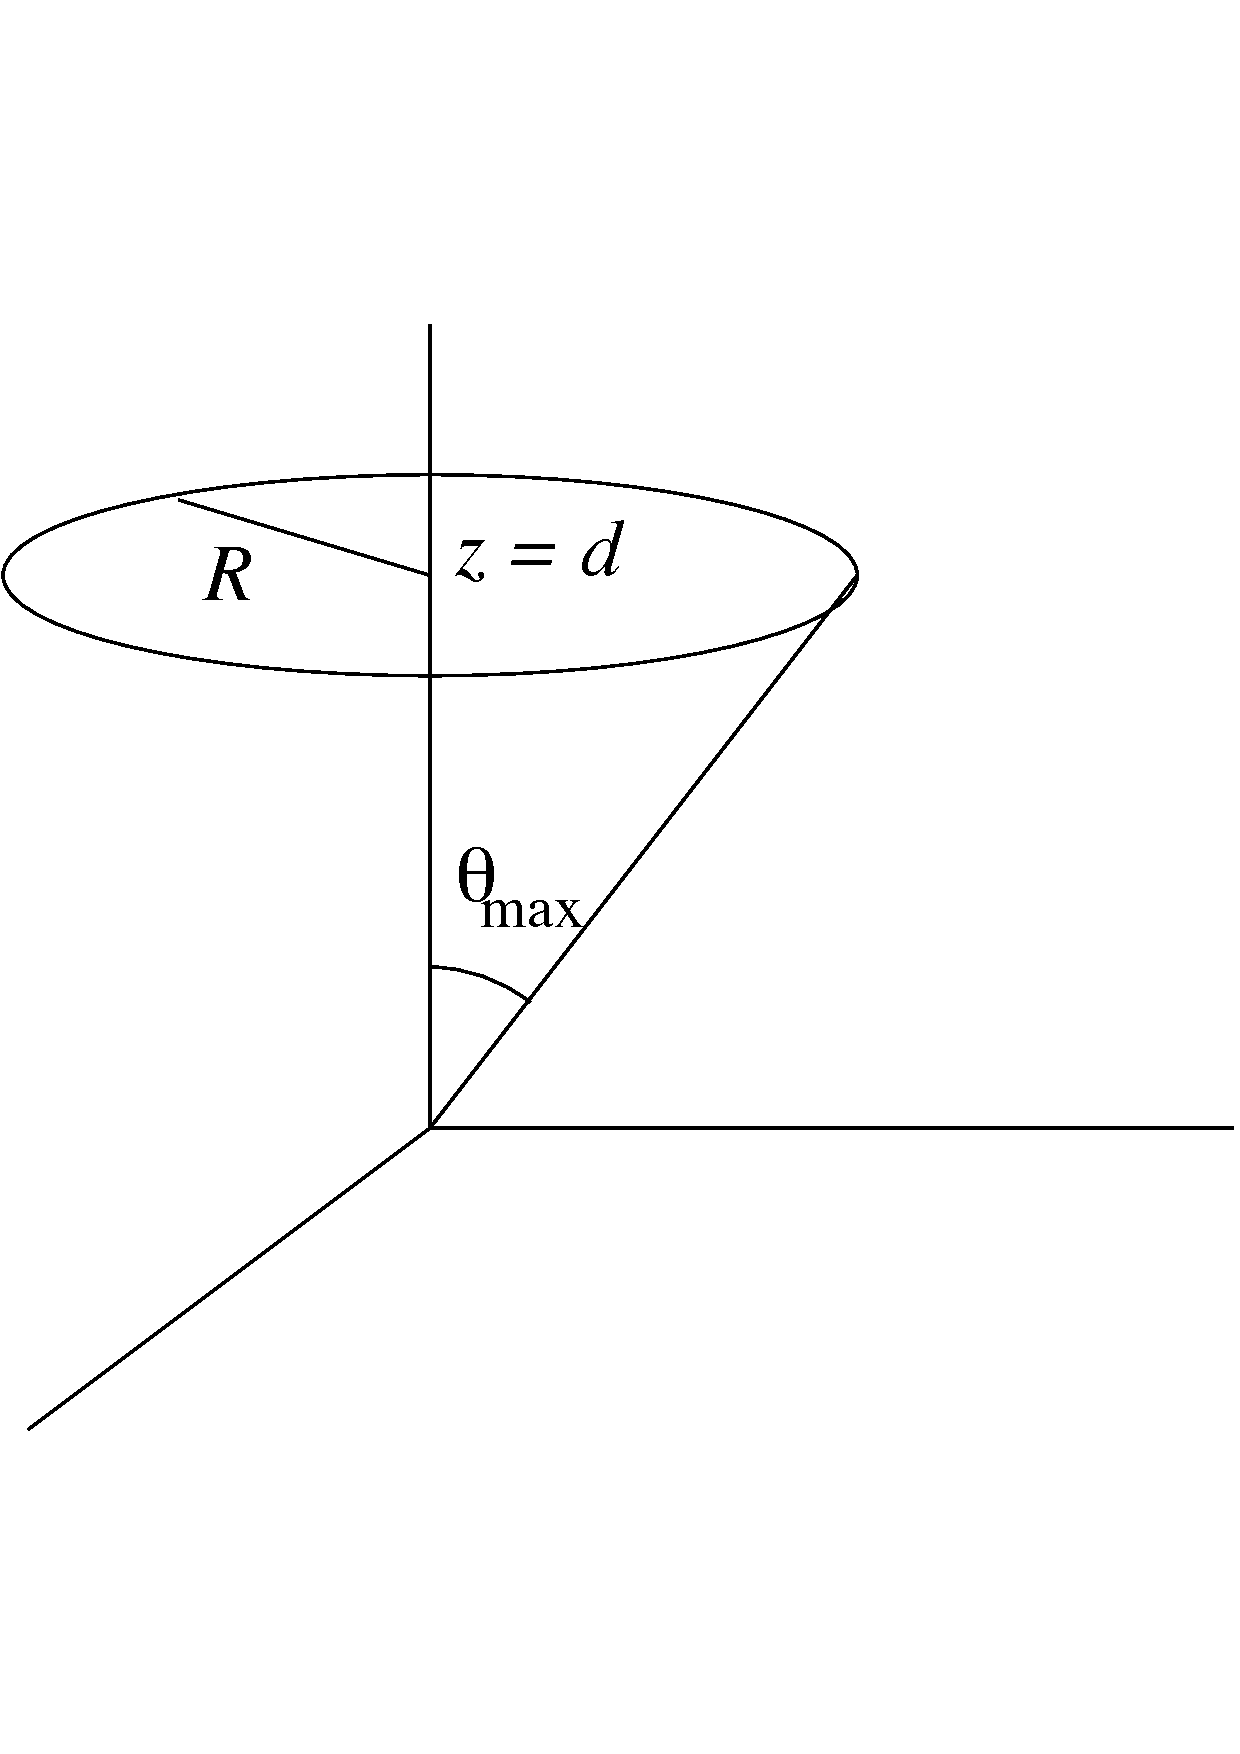
\includegraphics[width=6cm]{figs/schijf}
    \caption{A disc with radius~$R$.\label{fig:ex_schijf}}
    \end{SCfigure*}

\item Did you calculate the answer to question~a) in the right
way? If not, is it a good approximation? Do you have to use the
exact solution or is the approximate formula $\Omega = O / R^2$ a
good approximation?

\end{subvragen}

%%%%%%%%%%%%%%%%%%%%%%%%%%%%%%%%%%%%%%%%%%%%%%%

%%%%%%%%%%%%%%%%%%%%%%%%%%%%%%%%%%%%%%%%%%%%%%%%%%

\opgave{Camera obscura} 

Photo-film or CCD-cameras measure flux; to measure intensity one has
to constrain the directions from which radiation can reach the
film. One can use a camera obscura to achieve this. A camera obscura
consists of a rectangular box with a small hole (see
Fig.~\ref{fig:camera}). The hole has a diameter~$d$. The distance
between hole and film-surface is~$L$.

\begin{SCfigure*}
     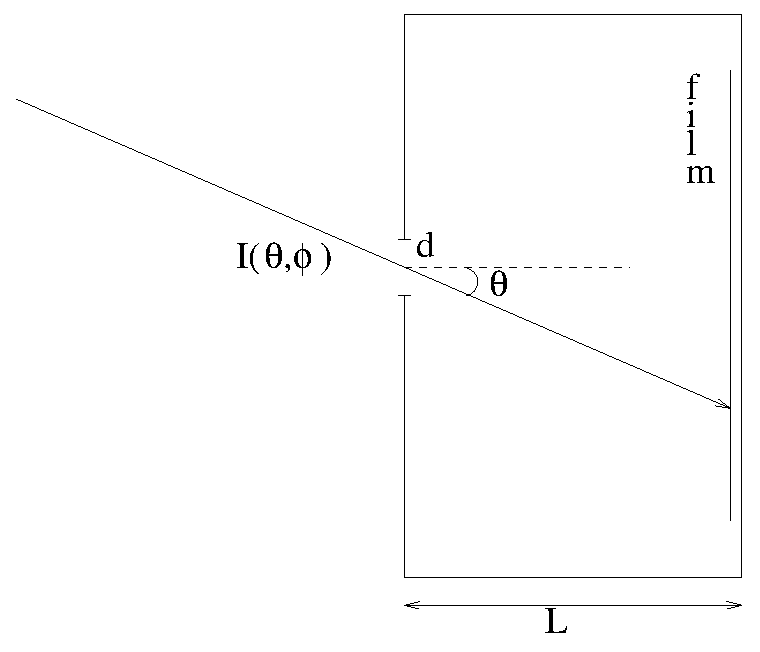
\includegraphics[width=6cm]{figs/camera}
    \caption{Camera obscura} \label{fig:camera}
\end{SCfigure*}

Show that the flux ${\cal F}_{\nu}$ on the film depends on the
intensity $I_{\nu}(\theta,\varphi)$ outside the camera in the
following way:

 % -
 \begin{equation}
     \label{eq:flux-camera}
     {\cal F}_\nu = \frac{\pi}{4} f^{2} I_\nu(\theta,\varphi) \cos^4 \theta ,
 \end{equation}
 % -

where $f=d/L$. (Hint: first show that the hole subtends a solid
angle~${\pi \over 4} f^2 \cos^3 \theta$ as seen from a point on the
film.)

The flux measured by the film is linearly dependent on the intensity
from the direction~$(\theta,\phi)$. On the one hand one wants to have a
small $f$, why? On the other hand $f$ should not be to small, why?

%%%%%%%%%%%%%%%%%%%%%%%%%%%%%%%%%%%%%%%%%%%%%%%%%%

%%%%%%%%%%%%%%%%%%%%%%%%%%%%%%%%%%%%%%%%%%%%%%%%%%%%%%
\opgave{Sharp-edged Sun}
%%%%%%%%%%%%%%%%%%%%%%%%%%%%%%%%%%%%%%%%%%%%%%%%%%%%%%

The Sun has a sharp edge when viewed at wavelengths in the optical continuum, but it does not have a clearly defined surface as it is made of gas. The sharp edge is therefore caused by a rapid decrease in optical thickness of the Sun close to the edge. The geometry of the problem is shown in Figure~\ref{fig:sharp-edge-star}. The optical thickness of of the Sun at a distance $y$ from the solar center (along the dashed line) is given by
\be
\taunu(y) = 2 \int_0^\infty \alpha_\nu(x,y) \, \dd x,
\ee
with $\alpha_\nu(x,y)$ the extinction coefficient at position $(x,y)$.

\begin{SCfigure*}
     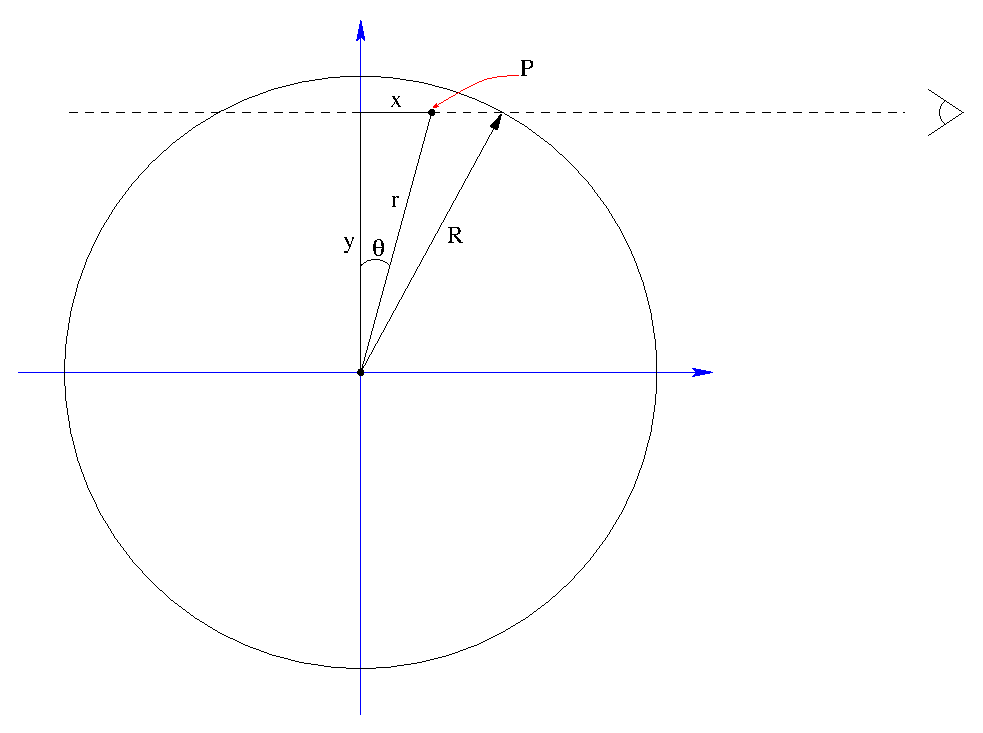
\includegraphics[width=10cm]{figs/sharp-edge-star}
    \caption{Geometry of the sharp-edged Sun problem.}  \label{fig:sharp-edge-star}
\end{SCfigure*}

\begin{enumerate} [label=(\alph*)]
\item
Show that in spherical coordinates

\begin{equation}
\tau_\nu(y) = 2 \int_y^\infty \alpha_\nu(r)  \frac{r}{\sqrt{r^2-y^2}} \, \dd r
\end{equation}

\item Now we need to specify the extinction coefficient as a function of $r$. We will simplify and assume that the solar atmosphere is isothermal. Then the density profile of the sun close to the visible surface at $r=R$ is given by
\be
\rho(r) = \rho_0 \exp^{(r-R)/h},
\ee
with \be
h = \frac{kT}{mg}
\ee
the pressure scale height and $\rho_0$ the density at $r=R$.

Compute the pressure scale height in km assuming $T=5000$~K, the average particle mass $m= m_\mathrm{H}$ and the gravity at the solar surface $g=GM_\odot / R^2$

\item Assume a constant opacity per mass unit $\kappa_\nu$. Then show that 
\be
\frac{\tau_\nu(y_1)}{\tau_\nu(y_2)} =  \frac{K_1(\frac{y_1}{h})}{K_1(\frac{y_2}{h})}
\ee
for two different heights $y_1$ and $y_2$. You can use
\be
\int_y^\infty \frac{r \, \exp^{-r/h} }{\sqrt{r^2-y^2}} \, \dd r = y \, \, K_1(\frac{y}{h}),
\ee
where $K_n$ is the modified Bessel function of the second kind.

\item Use Wolfram Alpha\footnote{\url{http://www.wolframalpha.com}} or a similar mathematics program to estimate the height difference $y_1-y_2$ so that 
$\tau_\nu(y_1) / \tau_\nu(y_2) = 0.01$, where $y_2=R$. Over this height difference the optical thickness along the line of sight will drop from 10 to 0.1, and is thus a reasonable measure of the sharpness of the solar limb.
In reality the temperature decreases with height in the solar photosphere, and the H$^-$ number density, which dominates the opacity decreases sharply with decreasing temperature. The solar limb is thus even sharper than you just computed.

\end{enumerate}

\end{opgaven}

\bibliographystyle{aa}
\bibliography{AS7006_ln}


\end{document}

%When there are multiple processes that contribute to  the emissivity and extinction coefficient then the source function is
%\be
%\Snu = \frac{\sum \jnu}{\sum \anu},
%\ee
%where the sums are taken over all relevant processes, and normally all processes add both to \jnu\ and to \anu.
